\Opensolutionfile{solution_file}[sols_all]
% в квадратных скобках фактическое имя файла

\section{Однородные функции}

\begin{problem}
Find the values $a$ and $b$ such that the function $f$ is homogeneous:

\[f(x,y)=2x^{b-a} y^{b+2} +y^{a+1} x^{-3b} +y^{7b} x^{-2a} .\]

For the values $a$ and $b$ you have found expand the function

\[h(x)=\sqrt{1+f(x,x)} \cdot (1-\cos (f(x,x))\]

as a power series up to $x^{4} $. State the range for $x$ where your expansion is correct. (Spring mock, 2012).



\begin{sol}
Функция $f(x,y)$ называется однородной степени однородности $m$, если для любого $t>0$ и для любых $x,y$ из области определения функции $f$, выполнено $f(tx,ty)=t^{m} f(x,y)$. Функция, заданная формулой в условии задачи является многочленом от двух переменных, состоящим из трех слагаемых. Каждое из слагаемых -- однородная функция автоматически, но для того чтобы сумма была однородной, необходимо и достаточно, чтобы однородность всех трех слагаемых была одной степени, откуда получаем систему уравнений

\[b-a+b+2=a+1-3b=7b-2a,\]

решением которой является $a=3,  b=1$. Тогда $f(x,x)=4x$. Разложим по формуле Тейлора $1-\cos (4x)$ до члена $x^{4} $. Мы получим
\[
1-\cos (4x)=8x^{2} -\frac{32}{3} x^{4} +\ldots,
\]
и так как это разложение начинается с $x^{2} $, то нам достаточно разложить $\sqrt{1+4x} $ до члена с $x^{2} $. Окончательно получаем
\begin{multline}
\sqrt{1+4x} \cdot (1-\cos (4x))=(1+2x-2x^{2} +\ldots )(8x^{2} -\frac{32}{3} x^{4} + \ldots )=8x^{2} +16x^{3} -\frac{80}{2} x^{4} +\ldots,
\end{multline}

или, используя запись остатка в форме Пеано $h(x)=8x^{2} +16x^{3} -\frac{80}{2} x^{4} +o(x^{4} )$.
\end{sol}
\end{problem} 


\begin{problem}
The homogeneous function $f$ is given by the equation

\[
f(x,y)=\int _{0}^{xy^{a} }(t^{3} +xt)dt .
\]


Find the value of the parameter $a$ and the degree of homogeneity of $\frac{\partial f}{\partial x} $. (Spring mock 2013).



\begin{sol}
Функция $f(x,y)$ находится интегрированием $f=\frac{1}{4} x^{4} y^{4a} +\frac{1}{2} x^{3} y^{2a} $. Оба слагаемых должны иметь одинаковую однородность, т.е. $4+4a=3+2a$, откуда $a=-\frac{1}{2} $. Тогда степень однородности функции $f(x,y)$ равна 2. Однородность любой из ее первых производных будет на единицу меньше, т.е. 1.
\end{sol}
\end{problem}




\section{Оптимизация с ограничениями в виде неравенств. Условия Куна-Таккера.}

\begin{problem}
Consider the monopolist producing two distinct goods. The cost function is given by $TC(q_{1} ,q_{2} )=q_{1} +kq_{2} $, where the constant $k\in (0;1)$. And the demand functions are given by $q_{1} (p_{1} ,p_{2} )=q_{2} (p_{1} ,p_{2} )=(p_{1} p_{2} )^{-3} $, where $p_1>0$ and $p_2>0$.

\begin{enumerate}
\item Find the optimal production bundle for the monopolist.
\item For which values of  $k$ one of the products is priced under marginal cost? (Spring mock, 2012).
\end{enumerate}



\begin{sol}
Хотя эта задача относится к теме «Безусловная оптимизация», но авторы пособия решили привести ее решение по двум причинам: с целью повторения темы, рассмотренной в курсе «Математика для экономистов» и в виду того, что трудность этой задачи превышает принятую в курсе «матэка».

Запишем задачу монополиста по максимизации прибыли:

$\pi =\frac{p_{1} +p_{2} -1-k}{(p_{1} p_{2} )^{3} } \to \max $. Прибыль здесь максимизируется по ценам $p_{1} ,p_{2} >0$. Выписывая условия первого порядка $\frac{\partial \pi }{\partial p_{1} } =0$ и $\frac{\partial \pi }{\partial p_{2} } =0$, и решая систему, получаем значения равновесных цен $p_{1} =p_{2} =\frac{3}{5} (1+k)$. Затем вычисляем производные второго порядка $\pi _{11} $, $\pi _{22} $ и $\pi _{12} =\pi _{21} $ при $p_{1} =p_{2} =\frac{3}{5} (1+k)$. Чтобы облегчить вычисление этих производных, лучше всего представить прибыль в виде суммы трех дробей:
\[
\pi =\frac{1}{p_{1}^{2} p_{2}^{3} } +\frac{1}{p_{1}^{3} p_{2}^{2} } -\frac{1+k}{p_{1}^{3} p_{2}^{3} }
\]
Гессиан при равновесных ценах является отрицательно определенным, что означает выполнение достаточного условия максимизации. Чтобы ответить на второй вопрос задачи следует рассмотреть по отдельности два двойных неравенства

(1) $1\le \frac{3}{5} (1+k)<k$ и (2) $k\le \frac{3}{5} (1+k)<1$. Неравенства получены из сопоставления цен с предельными издержками по первому и второму товарам $\frac{\partial TC}{\partial q_1}=1$, $\frac{\partial TC}{\partial q_2}=k$.


Решением первого из них является пустое множество, а решением второго --- $k < \frac{2}{3} $. Окончательный ответ: $k < \frac{2}{3} $.

С точки зрения микроэкономики, хотя производство второго товара становится при таком $k$ невыгодным, но убыток от его производства покрывается прибылью от производства первого товара.
\end{sol}
\end{problem}


\begin{problem}
Using the Lagrange multiplier method without reducing the number of variables by substitution find the minimum of the function

\[f(x,y,z)=2x^{2} +4y^{2} +xy+8z^{2} +2yz\]

subject to $x+y+\frac{3}{2} z\ge \frac{6}{5} $ and $x+y+z=1$. Check a sufficiency condition. (Spring mock 2012).


\begin{sol}
Проверка NDCQ тривиальна, т.к. ранг матрицы Якоби, составленной на основе ограничений, является полным, т.е. равняется 2. В самом деле, $J=\left(\begin{array}{c} {\begin{array}{ccc} {1} & {1} & {3/2} \end{array}} \\ {\begin{array}{ccc} {1} & {1} & {1} \end{array}} \end{array}\right)$.

Преобразуем ограничения задачи к более простому виду, однако, как предписано условием, не уменьшая число неизвестных:

\[
\begin{cases}
z\ge \frac{2}{5} \\
x+y+z=1.
\end{cases}
\]

Составим функцию Лагранжа задачи. $L=2x^{2} +4y^{2} +xy+8z^{2} +2yz+\lambda (1-x-y-z)+\mu (\frac{2}{5} -z)$. Тогда условия первого порядка будут выглядеть

\[
\begin{array}{l}
{\frac{\partial L}{\partial x} =4x+y-\lambda =0,} \\
{\frac{\partial L}{\partial y} =8y+x+2z-\lambda =0,} \\
{\frac{\partial L}{\partial z} =16z+2y-\lambda -\mu =0,} \\
{\mu \ge 0,  \mu (2/5-z)=0,  z\ge 2/5,  x+y+z=1.}
\end{array}
\]

Рассмотрим 2 случая: 1) пусть ограничение в виде неравенства не активно, т.е.$z>\frac{2}{5} $. Тогда $\mu =0$, и систему линейных уравнений относительно неизвестных $x,y,z,\lambda $ можно решить, например, методом Гаусса. Вычисления дают $z=1/7$, значение, не удовлетворяющее ограничению. Во втором случае полагаем $z=\frac{2}{5} $. Тогда решив систему относительно $x, y, \lambda, \mu $, получаем значения  $x=1/2$, $ y=1/10$. Осталось проверить, будет ли точка $(1/2,1/10,2/5)$ решением задачи.

%Для проверки достаточного условия минимизации, найдем окаймленный Гессиан функции Лагранжа. Он равен
%$\bar{H}=
%\left(\begin{array}{ccc}
%0 &  1   &  1 \\
%1 & {4} & {1} \\
%1 & {1} & {8} \\
%\end{array}\right)$. Знак определителя $\bar{H}$ отрицательный.

Для проверки достаточного условия минимизации поступим таким образом --- проверим, что функция $f(x,y,2/5)$ является выпуклой для всех $x,y$. Ее гессиан равен $H=\left(\begin{array}{cc} {4} & {1} \\ {1} & {8} \end{array}\right)$, а эта матрица положительно определенная. Следовательно, функция Лагранжа, рассматриваемая при $z=2/5$, также будет выпуклой по переменным $x$, $y$, $\lambda$.

%Таким образом, она является также вогнутой на выпуклом множестве, заданном ограничением $x+y+2/5=1$.

Однако, критическая точка выпуклой функции является точкой минимума этой функции, отсюда следует, что $(1/2, 1/10, 2/5)$ является точкой минимума $f(x,y,2/5)$ при наличии ограничения $x+y=3/5$.

Соответственно, минимальное значение функции, заданной на множестве, определенном ограничениями, равняется  $\frac{39}{25} $.
\end{sol}
\end{problem}


\begin{problem}
Use Lagrange multipliers method to solve optimization problem

\[xy\to \max \]

subject to $x\ge 0,  0\le y\le 3,  x+2y\le 8,  y\ge \frac{x^{2} }{16} +1$. (Exam, 2012).


\begin{sol}
Проверка NDCQ в этой задаче не вызывает трудностей. Градиенты ограничений на границе допустимого множества нигде не обращаются в ноль, а если составить якобиан, порожденный двумя ограничениями, то его ранг равен 2. В этой задаче, всего с учетом неотрицательности переменных, 5 ограничений в виде неравенств. При использовании метода Куна-Таккера нам понадобятся только 3 множителя Лагранжа  вместо пяти.


Кроме того, поскольку мы решаем задачу на максимум, то нулевые значения переменных в качестве критических точек не годятся (иначе данная целевая функция обратится в ноль). С учетом сказанного, мы введем функцию Лагранжа $L=xy+\lambda (3-y)+\mu (y-\frac{x^{2} }{16} -1)+\gamma (8-x-2y)$. Множество, на котором ищется максимум, является компактом, заданным неравенствами $\left\{\right. x\ge 0,  0\le y\le 3,  x+2y\le 8,  y\ge \frac{x^{2} }{16} +1\left. \right\}$. Легко видеть, что функция принимает максимальное значение только на границе этой области, т.к. внутри ее градиент всюду отличен от нуля. Тогда разобьем границу на три участка: (1) $\left\{y=3,  0\le x\le 2\right\}$, (2) $\left\{x+2y=8,  2\le x\le 4\right\}$ и (3) $\left\{y=\frac{x^{2} }{16} ,  0\le x\le 4\right\}$. Участки (1) и (2) имеют общую точку $(2,3)$, а участки (2) и (3) общую точку $(4,2)$. Выпишем условия Куна-Таккера с учетом положительности $x$и $y$:

\[\begin{array}{l} {\frac{\partial L}{\partial x} =y-\mu \frac{x}{8} -\gamma =0,} \\ {\frac{\partial L}{\partial y} =x-\lambda +\mu -2\gamma =0,} \\ {\gamma ,\mu ,\lambda \ge 0,  \mu (y-\frac{x^{2} }{16} -1)=0,  \gamma (8-x-2y)=0,  \lambda (3-y)=0.} \end{array}\]

\[x\ge 0,  0\le y\le 3,  x+2y\le 8,  y\ge \frac{x^{2} }{16} +1.\]

Будем искать критические точки лагранжиана на каждом из участков по отдельности. На участке (1) $\mu =\gamma =0$, поэтому мы получим $y=0$, что не может являться решением (см. выше). Аналогично, на участке (3)  $\gamma =\lambda =0$, откуда $x+\mu =0$, что также не дает решений. Остался участок (2).  Получим систему

\[\begin{array}{l} {y-\gamma =0,} \\ {x-2\gamma =0,} \\ {x+2y=8.} \end{array}\]

В качестве решения получаем точку $(4,2)$. Нами, правда, не исследована еще точка $(2,3)$, лежащая на границе первого и второго участков. Но она не может быть критической точкой лагранжиана, т.к. иначе мы получили бы $\lambda =-4$ (проверьте самостоятельно). По теореме Вейерштрасса данная функция принимает наибольшее значение на данном множестве, стало быть, найденная точка является решением задачи (точка глобального максимума). В этой точке функция принимает значение, равное 8.
\end{sol}
\end{problem}

\begin{problem}
A two-product monopoly seeks to maximize its profit. The revenue follows the formula $R(x,y)=6x-x^{2} +y-y^{2} $. The total costs function is given by $C(x,y)=x^{2} +y^{2} +4x+3y$, where $x$ and $y$ are outputs. State the problem of the monopoly, given condition that its profit $\pi =R-C$ should always remain nonnegative. Apply the Kuhn-Tucker conditions. Use Weierstrass theorem to confirm sufficiency. (Exam, 2013).


\begin{sol}
Сформулируем задачу монополиста.

\[\pi =2x-2y-2x^{2} -2y^{2} \to \max \]

при условии, что $x,y\ge 0,  2x-2y-2x^{2} -2y^{2} \ge 0.$

NDCQ выполнено, т.к. градиент ограничения $(2-4x,-2-4y)$ обращается в 0 при отрицательном значении $y$. Выпишем лагранжиан задачи $L=(1-\lambda )(2x-2y-2x^{2} -2y^{2} )$. Условия Куна-Таккера таковы

\[\begin{array}{l} {(1-\lambda )(2-4x)\le 0,\, x(1-\lambda )(2-4x)=0,} \\ {(1-\lambda )(-2-4y)\le 0,  y(1-\lambda )(-2-4y)=0,  \lambda \ge 0,  \lambda (2x-2y-2x^{2} -2y^{2} )=0,} \end{array}\]

кроме того, должны быть выполнены ограничения $x,y\ge 0,  2x-2y-2x^{2} -2y^{2} \ge 0.$

Из уравнения $y(1+\lambda)(-2-4y)=0$ сразу следует, что $y=0$. Тогда $x=1/2$ и из условия дополняющей нежесткости $\lambda(2x-2y-2x^2-2y^2)=0$ при подстановке комбинации выпусков $(x,y)=(\frac{1}{2} ,0)$, получаем  $\lambda =0$.

Множество, заданное неравенствами является компактом (представляет собою сегмент круга), поэтому применение теоремы Вейерштрасса возможно и найденная критическая точка является точкой максимума.
\end{sol}
\end{problem}

\begin{problem}
A price-taking firm has a total of $L$ units of labor (the only production factor it has) to allocate to the production of two goods. These can be sold at positive prices $p_{x} >0$ and $p_{y} >0$, respectively. Producing $x$ units of the first good requires $\alpha x^{2} $ units of labor, whereas producing  $y$ units of the second good requires $\beta y^{2} $ units of labor, where $\alpha$, $\beta >0$ are constants.

The firm seeks to maximize its revenue. Find what output levels of the two goods the firm will choose by using its endowment of labor. Confirm that you found the maximizing outputs. (Retake 2011).


\begin{sol}
Сначала формализуем задачу $\left\{\begin{array}{c} {p_{x} x+p_{y} y\to \max ,} \\ {\alpha x^{2} +\beta y^{2} \le L,} \\ {x,y\ge 0.} \end{array}\right. $

Начнём с проверки NDCQ. На основе активных ограничений выпишем якобиан системы функций, задающих ограничения:

\[
\begin{pmatrix}
2\alpha x & 2\beta y \\
1 & 0 \\
0 & 1
\end{pmatrix}
\]

Активными могут быть только два из трёх ограничений. То есть исследованию возможного значения ранга подлежат две подматрицы (случай $x=y=0$ отпадает):
$J_1=\begin{pmatrix}
2\alpha x & 2\beta y \\
1 & 0
\end{pmatrix}$ и $J_2=\begin{pmatrix}
2\alpha x & 2\beta y \\
0 & 1
\end{pmatrix}$.
В обоих случаях это матрицы полного ранга, то есть их ранг равняется двум. Кроме того, градиент ограничения $\begin{pmatrix}
2\alpha x & 2\beta y
\end{pmatrix}$ отличен от нуля.

Будем решать методом Куна-Таккера. Выпишем лагранжиан Куна-Таккера $\Lambda =p_{x} x+p_{y} y+\lambda (L-\alpha x^{2} -\beta y^{2} )$. Условия первого порядка (необходимые) будут таковы

\begin{align}
\label{GrindEQ__1_} & \frac{\partial \Lambda }{\partial x} =p_{x} -2\lambda \alpha x\le 0 \text{ и } x(p_{x} -2\lambda \alpha x)=0, \\
\label{GrindEQ__2_}  & \frac{\partial \Lambda }{\partial y} =p_{y} -2\lambda \beta y\le 0 \text{ и } y(p_{y} -2\lambda \beta y)=0, \\
\label{GrindEQ__3_}  & \frac{\partial \Lambda }{\partial \lambda } =L-\alpha x^{2} -\beta y^{2} \ge 0 \text{ и } \lambda (L-\alpha x^{2} -\beta y^{2} )=0, \\
\label{GrindEQ__4_}  & \lambda ,x,y\ge 0.
\end{align}


Решение этой задачи может быть сведено к рассмотрению нескольких случаев.

Случай 1. Сначала мы проверим, что при оптимальных значениях $x$ и $y$ условие $\frac{\partial \Lambda }{\partial \lambda } =L-\alpha x^{2} -\beta y^{2} \ge 0$ выполняется как равенство, т.е. является активным. С экономической точки зрения это будет означать, что фирма использует весь свой запас труда. В самом деле, если предположить противное, то в силу условия дополняющей нежесткости $\lambda (L-\alpha x^{2} -\beta y^{2} )=0$ значение $\lambda $ будет равно нулю, но это невозможно, т.к. из \ref{GrindEQ__1_} и \ref{GrindEQ__2_} будет следовать неположительность цен на продукцию. Следовательно, справедливо  $L-\alpha x^{2} -\beta y^{2} =0$.

Случай 2. В этой части решения будем искать внутреннее решение, т.е. такое, что $x,y>0$.

При положительных $x$ и $y$, из условий дополняющей нежесткости \ref{GrindEQ__1_} и \ref{GrindEQ__2_} будет следовать система уравнений

\begin{equation}
\begin{cases}
p_{x} -2\lambda \alpha x=0 \\
p_{y} -2\lambda \beta y=0
\end{cases}.
\end{equation}

Дополнив их уравнением $L-\alpha x^2-\beta y^2=0$, мы получим систему, решением которой являются

\begin{equation} \label{GrindEQ__7_}
\begin{cases}
x^*=p_{x} \sqrt{\frac{L}{\alpha p_{x}^{2} +\frac{\alpha ^{2} p_{y}^{2} }{\beta } } } , \\
y^*=p_{y} \sqrt{\frac{L}{\frac{\beta ^{2} p_{x}^{2} }{\alpha } +\beta p_{y}^{2} } }
\end{cases}
\end{equation}

Случай 3. Осталось рассмотреть возможность угловых решений, т.е. таких, что или $x=0$, или $y=0$ (одновременно $x$ и $y$ не могут обращаться в 0). Угловых решений в данной задаче быть не может, т.к. иначе бы одна из цен стала бы неположительной.

Почему же найденная критическая точка \ref{GrindEQ__7_} является точкой максимума? Обосновать это проще всего, опираясь на теорему Вейерштрасса о достижении функцией, непрерывной на компакте, своего наибольшего и наименьшего значений. Очевидно, наименьшее значение выручки равняется нулю, а наибольшее достигается в единственной критической точке. То, что множество допустимых значений является компактом, легко следует из того, что неравенства, задающие его, являются нестрогими, кроме того, геометрически на декартовой плоскости граница этого множества представляет собой четверть эллипса и два отрезка координатных осей, т.е. допустимое множество ограничено.
\end{sol}
\end{problem}


\begin{problem}
Find the global maximum of the objective function $x^{2} +4y^{2} +z^{2} $ subject to constraints $x+y+z\le 12, x,y,z\ge 0$. Use Kuhn-Tucker conditions. Verify maximization by applying the Weierstrass theorem or otherwise. (Exam 2009).


\begin{sol}

Проверку NDCQ мы предлагаем провести читателю самостоятельно. В этой задаче проверка не представляет трудностей, потому что все активные ограничения являются линейными.


Исследование на глобальный максимум мы проводим по той же схеме, что и на локальный максимум. Отличие будет состоять в том, что после нахождения всех критических точек, нам нужно будет вычислить значения целевой функции во всех этих точках, и выбрать точку, где функция принимает самое большое значение.

Метод решения Куна-Таккера предполагает формирование лагранжиана в виде $L=x^{2} +4y^{2} +z^{2} +\lambda (12-x-y-z)$. Тогда условия Куна-Таккера могут быть выписаны

\begin{align*}
\frac{\partial L}{\partial x} =2x-\lambda \le 0, \, x(2x-\lambda )=0, \\
\frac{\partial L}{\partial y} =8y-\lambda \le 0, \, y(8y-\lambda )=0, \\
\frac{\partial L}{\partial z} =2z-\lambda \le 0, \, z(2z-\lambda )=0,  \\
x+y+z\le 12, \, x,y,z\ge 0 \text{ и } \lambda \ge 0.
\end{align*}

Перебирая разные случаи, как и при решении задачи 2.5, мы приходим к следующим выводам: система уравнений и неравенств, рассмотренная выше, имеет единственное внутреннее решение $x^*=z^*=\frac{16}{3} , y^*=\frac{4}{3} $; остальные 6 критических точек лежат либо в одной из координатных плоскостей (как, например, $x^*=0, y^*=\frac{12}{5} , z^*=\frac{48}{5} $), либо на одной из координатных осей (как, например, $x^*=0, y^*=12, z^*=0$).

Самое большое значение функция принимает в угловой точке с координатами $x^*=0, y^*=12, z^*=0$, и это значение равно 576.
\end{sol}
\end{problem}



\section{Линейное программирование}

\begin{problem}
For any real number $\lambda $, find the minimal value of the objective function $x_{1} +6x_{2} +2x_{3} +4x_{4} $, subject to the constraints $\lambda x_{1} +x_{2} -x_{3} +x_{4} \ge -1,  x_{1} +\frac{3}{2} x_{2} +x_{3} +x_{4} \ge 5,$ all choice variables are nonnegative. (Exam, 2013).



\begin{sol}
Сформулируем двойственную задачу. Матрица ограничений исходной задачи имеет вид $A=\left(\begin{array}{c} {\begin{array}{cccc} {\lambda } & {1} & {-1} & {1} \end{array}} \\ {\begin{array}{cccc} {1} & {3/2} & {1} & {1} \end{array}} \end{array}\right)$. В двойственной задаче будет максимизироваться функция $-y_{1} +5y_{2} $ по неотрицательным двойственным переменным, удовлетворяющим ограничениям, записанным в матричной форме $A^{T} \left(\begin{array}{c} {y_{1} } \\ {y_{2} } \end{array}\right)\le \left(\begin{array}{c} {1} \\ {6} \\ {2} \\ {4} \end{array}\right)$.

Изобразим допустимое множество на плоскости переменных $(y_{1} ,y_{2} )$ (см. рисунок), пока без учета неравенства $\lambda y_{1} +y_{2} \le 1$.



\tikzstyle{dot} = [circle, minimum width=3pt, fill, inner sep=0pt]
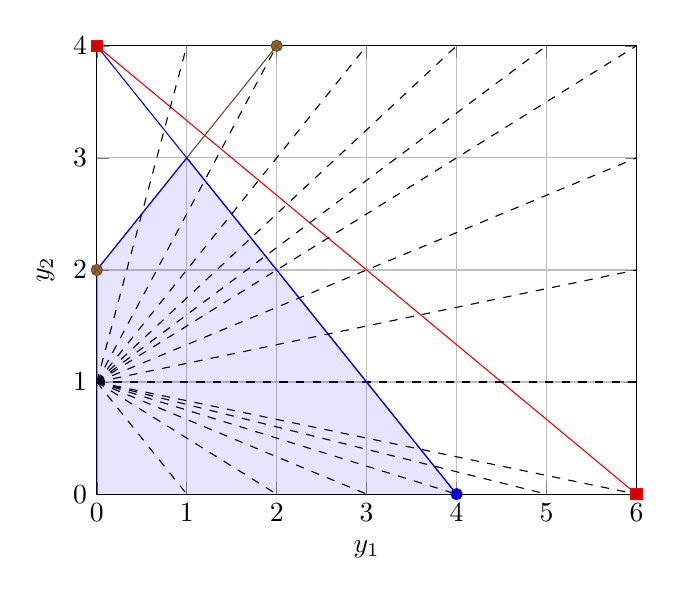
\begin{tikzpicture}
\begin{axis}[ grid=major,
xmin=0, xmax=6, ymin=0, ymax=4,xlabel={$y_1$},ylabel={$y_2$},
]
\addplot coordinates { (0,4) (4,0) };
\addplot coordinates { (0,4) (6,0) };
\addplot coordinates { (0,2) (2,4) };
\addplot [dashed, color=black] coordinates { (0,1) (1,4) };
\addplot [dashed, color=black] coordinates { (0,1) (2,4) };
\addplot [dashed, color=black] coordinates { (0,1) (3,4) };
\addplot [dashed, color=black] coordinates { (0,1) (4,4) };
\addplot [dashed, color=black] coordinates { (0,1) (5,4) };
\addplot [dashed, color=black] coordinates { (0,1) (6,4) };
\addplot [dashed, color=black] coordinates { (0,1) (6,3) };
\addplot [dashed, color=black] coordinates { (0,1) (6,2) };
\addplot [dashed, color=black] coordinates { (0,1) (6,1) };
\addplot [dashed, color=black] coordinates { (0,1) (6,0) };
\addplot [dashed, color=black] coordinates { (0,1) (5,0) };
\addplot [dashed, color=black] coordinates { (0,1) (4,0) };
\addplot [dashed, color=black] coordinates { (0,1) (3,0) };
\addplot [dashed, color=black] coordinates { (0,1) (2,0) };
\addplot [dashed, color=black] coordinates { (0,1) (1,0) };
\addplot [color=blue,fill=blue, fill opacity=0.1] coordinates
    { (0,0) (0,2) (1,3) (4,0) };
\end{axis}
\end{tikzpicture}

Уравнение $\lambda y_{1} +y_{2} =1$ при варьировании параметра $\lambda $ определяет пучок прямых проходящих через точку $(0,1)$. Без учета этого уравнения (неравенства из системы ограничений) допустимое множество представляет собою четырехугольник, заданный неравенствами $D=\left\{y_{1} ,y_{2} \ge 0,y_{1} +y_{2} \le 4,y_{2} \le 2+y_{1} \right\}$. В зависимости от знака $\lambda $ результирующим допустимым множеством будет являться либо часть множества $D$, лежащая над прямой $\lambda y_{1} +y_{2} =1$, или же под нею. Чтобы найти максимальное значение двойственной целевой функции, необходимо рассмотреть следующие диапазоны значений параметра $\lambda $: (1) $-\infty <\lambda \le -2,$ (2) $-2<\lambda \le 1/5,$ (3) $\lambda >1/5.$ Целевая функция принимает равные значения в точках прямой $-y_{1} +5y_{2} =C$, тем самым, выбирая наибольшее возможное значение $C$, мы сдвигаем посредством параллельного переноса прямую $y_{2} =\frac{1}{5} y_{1} $, до тех пор, пока она имеет хотя бы одну общую точку с допустимым множеством.


При значениях $\lambda $ из первого диапазона, максимум целевой функции достигается в вершине четырехугольника $D$, а именно в точке $(1,3)$. Тогда минимум целевой функции прямой (исходной) задачи равен 14. При росте значения $\lambda $, прямые из пучка, заданного $\lambda y_{1} +y_{2} =1$ поворачиваются вокруг общей вершины по часовой стрелке. В диапазоне (2) максимум достигается в точке пересечения прямых $\lambda y_{1} +y_{2} =1$ и $y_{1} +y_{2} =4$. Тогда оптимальное значение  равно $\frac{2-20\lambda }{1-\lambda } $, т.к. оно вычисляется в $(\frac{3}{1-\lambda } ,  \frac{1-4\lambda }{1-\lambda } )$. Наконец, для всех остальных значений $\lambda $ максимум достигается в $(0,1).$ Оно равно 5. По теореме двойственности, все найденные максимальные значения функции в двойственной задаче совпадают с минимальными значениями функции прямой задачи.
\end{sol}
\end{problem}

\begin{problem}
Consider the linear programming problem with parameter $\beta $ and nonnegative $x_{i} $, for all $i=1, 2, 3, 4$:

\[3x_{1} +x_{2} -x_{3} +4x_{4} \to \max ,\]

\[
\begin{cases}
x_{1} +x_{2} -x_{3} +x_{4} \le 1, \\
\beta x_{1} +x_{2} +x_{3} +2x_{4} \le 2.
\end{cases}
\]

\begin{enumerate}
\item  Find the optimal values of the primal variables for $\beta =6$.

\item  Find the function $\varphi (\beta )$, where $\varphi (\beta )$ is the maximum value of the objective function for fixed value of $\beta $.

\item  Sketch the graph of $\varphi (\beta )$.  (Exam, 2014).
\end{enumerate}



\begin{sol}
Сначала выпишем исходную задачу в матричной форме


\[3x_{1} +x_{2} -x_{3} +4x_{4} \to \max ,\]

\[\left(\begin{array}{c} {1} \\ {\beta } \end{array}\begin{array}{c} {1} \\ {1} \end{array}\begin{array}{c} {-1} \\ {1} \end{array}\begin{array}{c} {1} \\ {2} \end{array}\right)\left(\begin{array}{c} {x_{1} } \\ {x_{2} } \\ {x_{3} } \\ {x_{4} } \end{array}\right)\le \left(\begin{array}{c} {1} \\ {2} \end{array}\right), x_{i} \ge 0.\]

Двойственная задача будет выглядеть следующим образом

\[y_{1} +2y_{2} \to \min ,\]

$\left(\begin{array}{c} {1} \\ {1} \\ {-1} \\ {1} \end{array}\begin{array}{c} {\beta } \\ {1} \\ {1} \\ {2} \end{array}\right)$
$\left(\begin{array}{c} {y_{1} } \\ {y_{2} } \end{array}\right)\ge \left(\begin{array}{c} {3} \\ {1} \\ {-1} \\ {4} \end{array}\right)$, и $y_{1} , y_{2} \ge 0$.

Задачу лучше решать в таком порядке: изобразить допустимое множество на плоскости переменных $y_{1} ,y_{2} $ для всех возможных значений параметра $\beta $ (может оказаться так, что для некоторых значений этого параметра допустимое множество окажется пустым), а затем найти минимальное значение двойственной целевой функции на этом множестве, а потом, зафиксировав $\beta =6$, определить значения исходных переменных $x_{i} $, при которых достигается это минимальное значение.


\tikzstyle{dot} = [circle, minimum width=3pt, fill, inner sep=0pt]
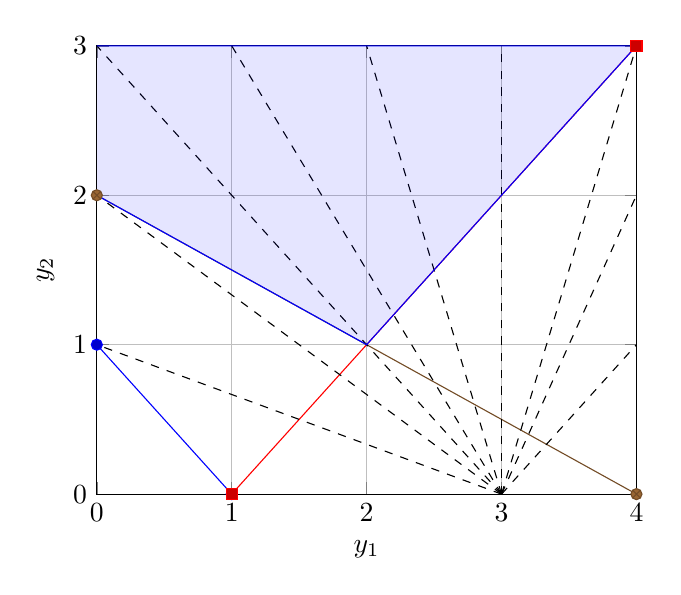
\begin{tikzpicture}
\begin{axis}[ grid=major,
xmin=0, xmax=4, ymin=0, ymax=3,xlabel={$y_1$},ylabel={$y_2$},
]
\addplot coordinates { (0,1) (1,0) };
\addplot coordinates { (1,0) (4,3) };
\addplot coordinates { (4,0) (0,2) };
\addplot [dashed, color=black] coordinates { (3,0) (0,1) };
\addplot [dashed, color=black] coordinates { (3,0) (0,2) };
\addplot [dashed, color=black]  coordinates { (3,0) (0,3) };
\addplot  [dashed, color=black] coordinates { (3,0) (1,3) };
\addplot [dashed, color=black] coordinates { (3,0) (2,3) };
\addplot  [dashed, color=black] coordinates { (3,0) (3,3) };
\addplot  [dashed, color=black] coordinates { (3,0) (4,3) };
\addplot  [dashed, color=black] coordinates { (3,0) (4,2) };
\addplot [dashed, color=black] coordinates { (3,0) (4,1) };
\addplot [color=blue,fill=blue, fill opacity=0.1] coordinates
    {  (0,2) (2,1) (4,3) (0,3) };
\end{axis}

\end{tikzpicture}


Ограничение $y_{1} +y_{2} \ge 1$ является несущественным, т.е. не влияющим на окончательный вид допустимого множества. Фактически множество представляет собой часть первого квадранта, граница которого является отрезками прямых $y_{1} +\beta y_{2} =3$, $y_{2} =y_{1} -1$, $y_{1} +2y_{2} =4$. При варьировании значения $\beta $, первая из указанных прямых поворачивается вокруг точки $(3,0)$. На рисунке проще сначала изобразить прямые, задаваемые уравнениями $y_{2} =y_{1} -1$ и $y_{1} +2y_{2} =4$. Они пересекаются в точке $A(2,1)$. Таким образом, если, предположим, прямая с уравнением  $y_{1} +\beta y_{2} =3$ пройдет ниже точки $A$, то для этих значений параметра минимум функции будет достигаться в точке $A$ и тогда он равняется 4. Очевидно, что такое прохождение прямой $y_{1} +\beta y_{2} =3$ соответствует значениям $\beta \ge 1$, ввиду того, что при $\beta =1$ прямая $y_{1} +\beta y_{2} =3$ пройдет через точку $A$, а при больших значениях $\beta $, эта прямая будет проходить ниже.

Теперь изучим двойственную задачу при $0<\beta <1$. В этом случае допустимое множество будет ограничено снизу прямой $y_{1} +\beta y_{2} =3$, и нам понадобится точка пересечения этой прямой с $y_{2} =y_{1} -1$, которую мы обозначим $B$. Ее координаты $\left(\frac{2}{\beta +1} +1,\frac{2}{\beta +1} \right)$. Искомое значение $\varphi (\beta )$ составит $\varphi (\beta )=\frac{6}{\beta +1} +1$. Интересно, что найденное значение $\varphi (\beta )$ останется верным при $\beta =0$ (при этом значении параметра прямая будет вертикальной), а также и при некоторых отрицательных значениях $\beta $. Легко увидеть, что $\varphi (\beta )=\frac{6}{\beta +1} +1$ годится также и для значений $-1<\beta <0$. При приближении значения $\beta $ к -1, точка $B$удаляется в бесконечность, что вполне согласуется с формулой $\varphi (\beta )=\frac{6}{\beta +1} +1$. Наконец, при $\beta \le -1$ допустимое множество вырождается в пустое, и $\varphi (\beta )$ не существует.

Окончательно,

\[\varphi (\beta )=\left\{\begin{array}{l} {+\infty , \beta \le -1} \\ {\frac{6}{\beta +1} +1, -1<\beta \le 1} \\ {4, \beta >1} \end{array}\right. \]

Осталось ответить на вопрос пункта а). Минимум двойственной функции достигается в точке $A$. В этой внутренней точке только два неравенства из четырех являются активными, а именно, $y_{2} =y_{1} -1$ и $y_{1} +2y_{2} =4$. Так как $y_{1}^{*} , y_{2}^{*} >0$, то, согласно первой теоремы двойственности, ограничения в первичной задаче являются активными, т.е. выполняются как равенства. Напротив, первые два ограничения двойственной задачи являются неактивными, что говорит о том, что $x_{1}^{*} =x_{2}^{*} =0$. Осталось найти $x_{3}^{*} $ и $x_{4}^{*} $ из решения системы уравнений $-x_{3} +x_{4} =1$ и $x_{3} +2x_{4} =2$, откуда $x_{3}^{*} =0$, $x_{4}^{*} =1$.

Проверим ответ пункта а). Поставим координаты найденной точки в исходную целевую функцию. Получим найденное ранее число 4.
\end{sol}
\end{problem}




\section{Дифференциальные и разностные уравнения}



%\textit{В этом разделе мы не рассматриваем упражнения по решению уравнений с постоянными коэффициентами и правой частью -- квазиполиномом, т.к. они разобраны в задачниках и пособиях по ДУ.}

\begin{problem}
The point elasticity of demand for a good is given by $\varepsilon =\frac{p^{2} }{p^{2} +4p+3} $. Find the demand function $q(p)$ given the initial condition $q(1)=1$. (Spring mock, 2012).



\begin{sol}
В условии задачи эластичность положительна, поэтому воспользуемся формулой эластичности с учетом знака $\varepsilon =-\frac{dq}{dp} \frac{p}{q} $. Нам нужно решить задачу Коши, проинтегрировав уравнение первого порядка с начальным значением.

\[-\frac{dq}{dp} \frac{p}{q} =\frac{p^{2} }{p^{2} +4p+3} , q(1)=1.\]

Это уравнение с разделяющимися переменными $-\int \frac{dq}{q} =\int \frac{pdp}{p^{2} +4p+3}   $. Представляя дробь $\frac{p}{p^{2} +4p+3} $ в виде суммы элементарных дробей $\frac{p}{p^{2} +4p+3} =\frac{-1/2}{p+1} +\frac{3/2}{p+3} $, интегрируем, оставляя константу интегрирования в виде множителя $q(p)=C\frac{\sqrt{p+1} }{(p+3)^{3/2} } $. Начальное условие позволяет определить константу $C=4\sqrt{2} $. Окончательно, $q(p)=\frac{4\sqrt{2} \sqrt{p+1} }{(p+3)^{3/2} } $.
\end{sol}
\end{problem}





\begin{problem}
Let $N(t)$ denote the size of population, $X(t)=\sqrt{N} $ being the total output in the economy. Consider the following model

\[\frac{\dot{N}}{N} =\alpha -\beta \frac{N}{X} ,\]

where $\dot{N}=\frac{dN}{dt} $ and $\alpha$, $\beta$ are some positive constants. Find  and explore its behavior as $t\to \infty $. (Spring mock, 2013).



\begin{sol}
Преобразуем уравнение к виду $\frac{dN}{N(\alpha -\beta \sqrt{N} )} =dt$, т.е. видим, что переменные разделились. Введя замену переменной $x=\sqrt{N} $, получаем интеграл
\[
\frac{2}{\alpha} \int \left( \frac{1}{x} + \frac{\beta}{\alpha - \beta x} \right) \, dx = \int \, dt.
\]

Можем проинтегрировать левую часть уравнения, тогда, возвращаясь к переменной $N$, получаем
\[
\frac{2}{\alpha } \ln \frac{\sqrt{N} }{\alpha -\beta \sqrt{N} } =t+C,
\]
где $C$ --- константа интегрирования. После ряда алгебраических операций получаем решение уравнения
\[
N(t)=\left(\frac{\alpha }{\beta +\gamma \exp (-\frac{\alpha }{2} t)} \right)^{2},
\]
где $\gamma$ --- константа, которую можно было бы определить, зная $N(0)$. Но в условии это значение не задано, поэтому оставим формулу как есть. При стремлении $t$ к бесконечности численность населения $N(t)$ стремится к $\left(\frac{\alpha }{\beta } \right)^{2} $, т.е. к конечному пределу.
\end{sol}
\end{problem}


\begin{problem}
Show that Chebyshev's equation $(1-x^{2} )y''-xy'+y=0$, where $\left|x\right|<1$, can be reduced to equation $\ddot{y}+y=0$ by substituting $x=\cos t$. Hence find the general solution of  Chebyshev's equation. (Exam 2013).


\begin{sol}
Используя формулы дифференцирования сложной функции, получаем  $y'=\frac{\dot{y}}{\dot{x}}=-\frac{\dot{y}}{\sin t}$,
\[
y''=\frac{1}{\sin t} \frac{d}{dt} \left( \frac{\dot{y}}{\sin t}  \right)=\frac{\ddot{y} \sin t - \dot{y} \cos t }{(\sin t)^3}.
\]

После подстановки в уравнение Чебышева, получаем  $\ddot{y}+y=0$. Общее действительное решение этого уравнения легко находится $y(t)=C_1 \sin t + C_2 \cos t$, где  $C_1$ и  $C_2$ --- произвольные константы. Возвращаясь к переменной $x$, получаем общее решение уравнения Чебышева $y=C_1 \sqrt{1-x^2} + C_2 x$, в виду того, что $\sin \arccos x=\sqrt{1-x^2}$.
\end{sol}
\end{problem}


\begin{comment} % old solution
Из замены $x=\cos t$ следует, что $1-x^2=\sin^2 t$, $\dot{y}=y'(-\sin t)$, $\ddot{y}=y'(-\cos t )+y'' \sin^2 t$.

Если к $\ddot{y}$ прибавить $y$, то мы получим исходное уравнение.
%Внимательно посмотрев на уравнение замечаем, что оно имеет вид $\ddot{y}+y=0$.

Находим корни характеристического уравнения $\lambda=\pm i$. Отсюда общее решение, как функция от $t$, имеет вид

\[
y(t)=C_1 \cos t + C_2 \sin t
\]

В данном случае $t=\pm \arccos x + 2\pi k$. После подстановки получаем:
\[
y(x)=C_1 \cos(\arccos x) + C_2 \sin (\arccos x)= C_1 x + C_2 \sqrt{1-x^2}
\]
\end{comment}



%\textit{Замечание. Боря, надо будет расширить название этого раздела, чтобы включить разностные уравнения и системы разностных уравнений. Кроме того, мне придется все же дать решения задач с постоянными коэффициентами и правой частью квазимногочленом, хотя в предыдущей версии я не собирался этого делать.}



\begin{problem}
Find the general solution of the differential equation $y''+2y'+y=xe^{-x} +\cos x$. (Exam 2012)


\begin{sol}
Составим характеристическое уравнение для однородного уравнения $y''+2y'+y=0$. Оно имеет вид $\lambda ^{2} +2\lambda +1=0$ и имеет единственный корень $\lambda =-1$ кратности 2. Тогда общее решение однородного уравнения определяется формулой $\tilde{y}(x)=C_{1} e^{-x} +C_{2} xe^{-x} $, где $C_{1} $ и $C_{2} $ произвольные вещественные константы.

Правая часть ДУ является квазимногочленом. При этом первое из слагаемых, входящих в правую часть, содержит $e^{-x} $, что говорит о том, что при выписывании частного решения неоднородного уравнения мы имеем дело с так называемым <<резонансным>> случаем. Если бы <<резонансного>> случая не было, то кандидатом на частное решение была бы функция $y_{1} (x)=(Ax+B)e^{-x} $, при этом $A, B$ - произвольные константы. Т.к. $\lambda =-1$ является корнем характеристического уравнения кратности 2, то выражение для $y_{1} (x)$ нужно умножить на $x^{2} $, т.е., пользуясь методом неопределенных коэффициентов, нам нужно искать константы $A, B$, подставляя в уравнение $y''+2y'+y=xe^{-x} $ функцию $(Ax^{3} +Bx^{2} )e^{-x} $, и после сокращения общего множителя $e^{-x} $ в этом уравнении, приравнять коэффициенты при одинаковых степенях $x$. После подстановки выражения с неопределенными коэффициентами в уравнение, приведения подобных членов, и сокращения экспоненты, мы получаем выражение $Ax+2B=x$, откуда $A=\frac{1}{6} $ и $B=0$.


Восстановим в правой части исходного уравнения $\cos x$, убрав $xe^{-x} $. Этот случай не является <<резонансным>>, поэтому, пользуясь, как и прежде, методом неопределенных коэффициентов, будем искать решение в виде $A\sin x+B\cos x$, подставляя это выражение в уравнение $y''+2y'+y=\cos x$, и приравнивая затем коэффициенты при $\sin x$ и $\cos x$. Находим $A=\frac{1}{2} $ и $B=0$.

Выписываем окончательный ответ $y(x)=C_{1} e^{-x} +C_{2} xe^{-x} +\frac{x^{3} }{6} e^{-x} +\frac{1}{2} \sin x$.
\end{sol}
\end{problem}

\begin{problem}
Find the general solution of the equation $y''''-5y'''+7y''-3y'=-4e^{x} $. Determine $y$ if $y(0)=3, y'(0)=5, y''(0)=14, y'''(0)=37.$ (Exam 2010)


\begin{sol}
Корни характеристического уравнения $\lambda ^{4} -5\lambda ^{3} +7\lambda ^{2} -3\lambda =0$ могут быть найдены следующим образом: после тривиального корня $\lambda _{1} =0, $ следующий корень уже кубического уравнения $\lambda ^{3} -5\lambda ^{2} +7\lambda -3=0$, находится подстановкой одного из делителей свободного члена, обычно эту проверку начинают с $\lambda _{2} =1$. Убедившись, что это корень уравнения, и поделив кубическое уравнение на $\lambda -1$, получаем в качестве делимого квадратный трехчлен $\lambda ^{2} -4\lambda +3$. Корнями квадратного уравнения являются $\lambda _{3} =1, \lambda _{4} =3$. Исходя из найденных корней, выписываем решение однородного уравнения $\tilde{y}(x)=C_{1} e^{x} +C_{2} xe^{x} +C_{3} +C_{4} e^{3x} $. Здесь мы сменили нумерацию корней и учли, что $\lambda =1$ является корнем кратности 2.

При подборе частного решения, учитываем, что имеем дело с <<резонансным>> случаем, т.к. правая часть уравнения  содержит $e^{x} $. Тогда кандидат на частное решение -- квазимногочлен $Ax^{2} e^{x} $ (из-за кратности корня $\lambda =1$ умножили на $x^{2} $). Подставляем $Ax^{2} e^{x} $ в исходное уравнение, приводим подобные члены, сокращаем на экспоненту, и окончательно приходим к уравнению $-4A=-4$, откуда $A=1$. Общее решение уравнения  имеет вид
\begin{equation} \label{eq:star}
y(x)=C_{1} e^{x} +C_{2} xe^{x} +C_{3} +C_{4} e^{3x} +e^{x}
\end{equation}
Решим задачу Коши. Для этого формула \ref{eq:star} должна быть продифференцирована в точке $x=0$ до трех раз, а затем составлена система уравнений относительно неизвестных $C_{1} , C_{2} , C_{3} , C_{4} $.

Мы получим систему

\[\begin{array}{c} {C_{1} +C_{3} +C_{4} +1=3,} \\ {C_{1} +C_{2} +3C_{4} +1=5,} \\ {C_{1} +2C_{2} +9C_{4} +1=14,} \\ {C_{1} +3C_{2} +27C_{4} +1=37.} \end{array}\]

Решением которой, как можно убедиться, является набор $\left(-\frac{3}{2} ,2,\frac{7}{3} ,\frac{7}{6} \right)$.
\end{sol}
\end{problem}

\begin{problem}
Solve differential equation $xy'+x^{2} +xy-y=0$. (Exam 2011)


\begin{sol}
Поделим уравнение на $x$, полагая, что $x\neq 0$. Если же $x=0$, то уравнение вырождается в $y=0$. Заметим, что в ходе интегрирования уравнения, мы получим общее решение, которое будет справедливо для всех $x$, потому что, как увидим, $y(0)=0$.

После деления уравнение может быть представлено в виде $y'+\frac{x-1}{x} y=-x$. Это уравнение линейное, неоднородное. Решать его можно разными способами. Например, можно воспользоваться методом вариации постоянной Эйлера. Суть метода состоит в следующем. Сначала отбрасывается правая часть уравнения, после чего уравнение легко интегрируется, т.к. переменные разделяются. В нашем случае мы получаем $\int \frac{dy}{y} =-\int \frac{x-1}{x} dx  $. После интегрирования находим $y(x)=Cxe^{-x} $. Теперь восстановим правую часть уравнения, считая что $C(x)$ --- функция, зависящая от $x$. Подставим функцию $y(x)=C(x)xe^{-x} $ в исходное уравнение. Мы получим $C'xe^{-x} =-x$. Откуда $C(x)=-e^{x} +\tilde{C}$. Здесь $\tilde{C}$ - произвольная константа. Окончательно получаем $y(x)=\tilde{C}xe^{-x} -x$.
\end{sol}
\end{problem}


\begin{problem}
 In the model of interacting inflation and unemployment based on the Phillips relation,  both unemployment rate $U$ and expected inflation $\pi$ are the solutions of the system $\dot{\pi}=\frac{3}{4}(p-\pi)$, $\dot{U}=-\frac{1}{2}(m-p)$, where $m$ is exogenously defined positive rate of nominal money growth and $p$ is the posteriori observed inflation satisfying equation $p=\frac{1}{6}-3U+\pi$.
\begin{enumerate}
\item Find the steady-state solutions for the inflation both expected and observed as well as the unemployment rate in terms of $m$.
\item Explore the dynamic stability of solutions.
\item What is the natural rate of unemployment?
\end{enumerate}



\begin{sol}
Используя формулу $p=\frac{1}{6}-3U+\pi$, приведем задачу к системе дифференциальных уравнений относительно неизвестных функций $\pi$, $U$:
\[
\begin{cases}
\dot{\pi}=-\frac{9}{4}U+\frac{1}{8} \\
\dot{U}=\frac{1}{2}\pi - \frac{3}{2}U+\frac{1}{12}-\frac{m}{2}
\end{cases}
\]

Матрица однородной системы уравнений имеет вид:
\[
A=\begin{pmatrix}
0 & -9/4 \\
1/2 & -3/2
\end{pmatrix}.
\]
Собственные значения этой матрицы  $\lambda_1=-\frac{3}{4}+i\frac{3}{4}$ и  $\lambda_1=-\frac{3}{4}-i\frac{3}{4}$. Собственный вектор, соответствующий $\lambda_1$  можно выбрать  равным
$\vec{a}=\begin{pmatrix}
3 \\
1-i
\end{pmatrix}$.

Умножив  $\exp \left(  \left(- \frac{3}{4} + i \frac{3}{4}  \right)t \right)$ на собственный вектор $\vec{a}$, и выделив вещественную и мнимую части произведения, выпишем общее решение однородной системы уравнений

\[
\begin{pmatrix}
\pi \\
U
\end{pmatrix} =
C_1 e^{-\frac{3}{4}t}
\begin{pmatrix}
3\cos \left( \frac{3}{4}t \right) \\
\cos \left( \frac{3}{4}t \right) + \sin \left( \frac{3}{4}t \right)
\end{pmatrix}
+
C_2 e^{-\frac{3}{4}t}
\begin{pmatrix}
3\sin \left( \frac{3}{4}t \right) \\
\sin \left( \frac{3}{4}t \right) - \cos \left( \frac{3}{4}t \right)
\end{pmatrix}.
\]
В этой формуле $C_1$  и $C_2$  --- произвольные константы.


Частное решение неоднородной системы будем искать в виде постоянного вектора
$
\begin{pmatrix}
\pi^* \\
U^*
\end{pmatrix}
$,
согласно методу неопределенных коэффициентов. Подстановка этого вектора в систему позволяет найти эти значения $\pi^*=m$ и  $U^*=1/18$.
Чтобы получить общее решение неоднородной системы, достаточно прибавить к общему решению однородной системы найденный вектор
$
\begin{pmatrix}
m \\
1/18
\end{pmatrix}
$. Решение, как видно, динамически устойчиво, потому что состоит из постоянной компоненты и экспоненциально затухающей части. Естественный уровень безработицы равен  $U^*=1/18$.
\end{sol}
\end{problem}

\begin{problem}
Find the general solution of the difference equation $y_{t+3} +y_{t+2} -2y_{t} =\frac{1+4^{t} }{2^{t} } $. (Exam 2010)


\begin{sol}
Сначала найдем общее решение однородного уравнения. Для этого выпишем характеристическое уравнение $b^{3} +b^{2} -2=0$. Один корень, а именно $b=1$ угадывается сразу, и после деления кубического многочлена на $b-1$ мы найдем делимое $b^{2} +2b+2$. Окончательно, $b_{1} =1, b_{2} =-1+i, b_{3} =-1-i$.

Общее решение однородного разностного уравнения, полученного обнулением правой части, будет иметь вид $y_{t} =C_{1} +C_{2} 2^{t/2} \cos \left(\frac{3\pi }{4} t\right)+C_{3} 2^{t/2} \sin \left(\frac{3\pi }{4} t \right)$. В этой формуле первое из слагаемых получено умножением произвольной константы $C_{1} $ на $1^{t} =1$, а два последующих слагаемых является линейной комбинацией вещественной и мнимой частей комплексного решения уравнения $(-1+i)^{t} $. При нахождении этих частей нам понадобилось записать корень характеристического уравнения в полярной форме $-1+i=\sqrt{2} \left(\cos \frac{3\pi }{4} +i\sin \frac{3\pi }{4} \right)$, затем возведя в натуральную степень $t$, воспользоваться формулой Муавра $\left(\cos \frac{3\pi }{4} +i\sin \frac{3\pi }{4} \right)^{t} =\cos \left(\frac{3\pi }{4} t \right)+i\sin \left(\frac{3\pi }{4} t \right)$, и, наконец, выделить вещественную и мнимую части.

Частное решение неоднородного уравнения будем искать методом неопределенных коэффициентов, при этом, пользуясь аналогией с поиском частных решений дифференциальных уравнений. Пусть $\tilde{y}_{t} =A \left(\frac{1}{2} \right)^{t} +B2^{t} $, где $A, B$ --- константы, находимые после подстановки выражения в исходное уравнения, и приравнивания коэффициентов при соответствующих показательных функциях. Т.к. ни 2, ни $\frac{1}{2} $ не являются корнями характеристического уравнения, то мы имеем дело с <<простым>>, а не <<резонансным>> случаем. Находим $A=-\frac{8}{13} $ и $B=\frac{1}{10} $.

Окончательный ответ
\[
y_{t} =C_{1} +C_{2} 2^{t/2} \cos \left(\frac{3\pi }{4} t \right)+
C_{3} 2^{t/2} \sin \left(\frac{3\pi }{4} t \right)-\frac{8}{13} \left(\frac{1}{2} \right)^{t} +\frac{1}{10} 2^{t}
\]
\end{sol}
\end{problem}


\begin{problem}
Solve the system of ODE
\[
\begin{cases}
\dot{x}=5x+3y, \\
\dot{y}=-3x-y.
\end{cases}
\]
(Exam 2011)


\begin{sol}
Системы дифференциальных уравнений второго порядка, как правило, могут быть легко сведены к уравнению второго порядка относительно одной из неизвестных функций, но мы попробуем решить эту систему другим методом, который применим к системам любого порядка.

Для решения нам следует найти собственные значения и соответствующие им собственные векторы матрицы системы $A=\left(\begin{array}{cc} {5} & {3} \\ {-3} & {-1} \end{array}\right)$. Собственные значения, $\lambda _{1} =\lambda _{2} =2$. Собственному значению кратности 2 соответствует единственный собственный вектор $e_{1} =\left(\begin{array}{c} {1} \\ {-1} \end{array}\right)$. Тем самым найдено одно из двух линейно независимых решений системы, а именно, функция $\left(\begin{array}{c} {x} \\ {y} \end{array}\right)=\left(\begin{array}{c} {1} \\ {-1} \end{array}\right)\exp (2t)$.


Матрицу второго порядка можно привести к нормальной жордановой форме, выбирая базис из собственных и присоединённых векторов.


Чтобы получить второе решение, найдём, так называемый, присоединенный вектор $e_{2} $, являющийся решением неоднородной алгебраической системы $Ae_{2} =\lambda e_{2} +e_{1} $. Конкретно в нашем случае, можно выбрать любой вектор $\left(\begin{array}{c} {\alpha } \\ {\beta } \end{array}\right)$, компоненты которого удовлетворяют уравнению $3\alpha +3\beta =1$, например, $e_{2} =\left(\begin{array}{c} {1/3} \\ {0} \end{array}\right)$. Таким образом, второе линейно независимое решение будет иметь вид $(te_{1} +e_{2} )\exp (2t)=\left(\begin{array}{c} {t+1/3} \\ {-t} \end{array}\right)\exp (2t)$.

Окончательно, решение
\[
\left(\begin{array}{c} {x} \\ {y} \end{array}\right)=C_{1} \left(\begin{array}{c} {1} \\ {-1} \end{array}\right)\exp (2t)+C_{2} \left(\begin{array}{c} {t+1/3} \\ {-t} \end{array}\right)\exp (2t)
\]

Проверим, что мы получим тот же ответ, решая систему сведением к одному уравнению.

Например, выразим $y=\frac{1}{3} (\dot{x}-5x)$ из первого уравнения, и подставим во второе $\frac{1}{3} (\ddot{x}-5\dot{x})=-3x-\frac{1}{3} (\dot{x}-5x)$. Упростив уравнение, получим $\ddot{x}-4\dot{x}+4x=0$. Его общее решение $x(t)=C_{1} e^{2t} +C_{2} te^{2t} $ (случай кратных корней). Тогда $y(t)=-C_{1} e^{2t} +\frac{1}{3} C_{2} e^{2t} -C_{2} te^{2t} $. Решая задачу с использованием присоединенного вектора, мы получили бы ровно такой же ответ, если бы выбрали другой присоединенный вектор $e_{2} =\left(\begin{array}{c} {0} \\ {-1/3} \end{array}\right)$.
\end{sol}
\end{problem}





\begin{problem}
Solve the system of differential equations
\[
\begin{cases}
\dot{x}=5x+3y+1, \\
\dot{y}=-3x-y.
\end{cases}
\]
(Retake exam 2013)



\begin{sol}
Найдем собственные значения и собственные векторы матрицы системы
$A=\begin{pmatrix}
5 & 3 \\
-3 & -1 \\
\end{pmatrix}$, решив квадратное уравнение
$
\begin{vmatrix}
5-\lambda & 3 \\
-3 & -1-\lambda
\end{vmatrix} = 0
$.
Получаем корень кратности 2, равный 2. Можем найти единственный собственный вектор  $\vec{e}_1=\begin{pmatrix}
1 \\
-1
\end{pmatrix}$.


Чтобы найти присоединенный вектор, следует решить неоднородную систему алгебраических уравнений $A\vec{e}_2=2\vec{e}_2+\vec{e}_1$, или
\[
\begin{pmatrix}
3 & 3 \\
-3 & -3 \\
\end{pmatrix}
\begin{pmatrix}
x_1 \\
x_2
\end{pmatrix} =
\begin{pmatrix}
1 \\
-1
\end{pmatrix}
\]


Подходит, например, вектор $\begin{pmatrix}
1/3 \\
0
\end{pmatrix}$.
Тогда общее решение однородной системы будет иметь вид
\[
\begin{pmatrix}
x(t) \\
y(t)
\end{pmatrix} =
C_1 e^{2t}
\begin{pmatrix}
1 \\
-1
\end{pmatrix}
+ C_2 e^{2t}
\begin{pmatrix}
t+1/3 \\
-t
\end{pmatrix}
\]
Чтобы получить второе линейно независимое решение, мы воспользовались формулой $e^{\lambda t }(t\vec{e}_1+\vec{e}_2)$. Правда, она лишь применима к системам второго порядка. Частное решение является постоянным вектором, который может быть найден методом неопределенных коэффициентов. Окончательно,
\[
\begin{pmatrix}
x(t) \\
y(t)
\end{pmatrix} =
C_1 e^{2t}
\begin{pmatrix}
1 \\
-1
\end{pmatrix}
+ C_2 e^{2t}
\begin{pmatrix}
t+1/3 \\
-t
\end{pmatrix}+
\begin{pmatrix}
1/4 \\
-3/4
\end{pmatrix}
\]
\end{sol}
\end{problem}

\begin{problem}
Solve the initial-value problem for the system of difference equations
\[
\begin{cases}
x_{t+1} =x_{t} +y_{t} , \\
y_{t+1} =3x_{t} -y_{t} -5,
\end{cases}
\]

where $x_{0} =y_{0} =0$. (Exam 2012).


\begin{sol}
Найдем собственные значения и собственные векторы матрицы системы
$A=\begin{pmatrix}
1 & 1 \\
3 & -1
\end{pmatrix}$. Получаем  $\lambda_1=2$, $\lambda_2=-2$, и, соответственно,
$\vec{e}_1=\begin{pmatrix}
1 \\
1
\end{pmatrix}$,
$\vec{e}_2=\begin{pmatrix}
1 \\
-3
\end{pmatrix}$. Ищем частное решение неоднородной системы в виде постоянного вектора
$\begin{pmatrix}
a \\
b
\end{pmatrix}$.
После подстановки в систему, получаем
$\begin{pmatrix}
5/3 \\
0
\end{pmatrix}$.
Наконец, используя начальные условия, выпишем окончательный ответ:
\[
\begin{pmatrix}
x_t \\
y_t
\end{pmatrix} =
-\frac{5}{4}
\begin{pmatrix}
1 \\
1
\end{pmatrix}
2^t
-\frac{5}{12}
\begin{pmatrix}
1 \\
-3
\end{pmatrix}
(-2)^t
+\begin{pmatrix}
5/3 \\
0
\end{pmatrix}
\]
\begin{comment} % old solution
Найдем сначала решение однородной системы уравнений $\left(\begin{array}{c} {x_{t+1} } \\ {y_{t+1} } \end{array}\right)=\left(\begin{array}{cc} {1} & {1} \\ {3} & {-1} \end{array}\right)\left(\begin{array}{c} {x_{t} } \\ {y_{t} } \end{array}\right)$. Находим собственные значения и собственные векторы матрицы системы $\lambda _{1} =2, e_{1} =\left(\begin{array}{c} {1} \\ {1} \end{array}\right)$ и $\lambda _{2} =-2, e_{2} =\left(\begin{array}{c} {1} \\ {-3} \end{array}\right)$. Общее решение однородной системы разностных уравнений имеет вид $\left(\begin{array}{c} {x_{t} } \\ {y_{t} } \end{array}\right)=C_{1} \left(\begin{array}{c} {1} \\ {1} \end{array}\right)2^{t} +C_{2} \left(\begin{array}{c} {1} \\ {-3} \end{array}\right)(-2)^{t} $,где $C_{1} $ и $C_{2} $ произвольные константы.


Правая часть исходной системы является постоянным вектором, поэтому подберем частное решение в виде постоянного вектора с неопределенными компонентами $\left(\begin{array}{c} {\alpha } \\ {\beta } \end{array}\right)$. Подставив его в систему, получим частное решение $\left(\begin{array}{c} {5/3} \\ {0} \end{array}\right)$.


Перейдем к решению задачи Коши. Для этого, выписав общее решение $\left(\begin{array}{c} {x_{t} } \\ {y_{t} } \end{array}\right)=C_{1} \left(\begin{array}{c} {1} \\ {1} \end{array}\right)2^{t} +C_{2} \left(\begin{array}{c} {1} \\ {-3} \end{array}\right)(-2)^{t} +\left(\begin{array}{c} {5/3} \\ {0} \end{array}\right)$, положим $t=0$, и приравняем правый столбец решения начальным данным. Из решения системы находим $C_{1} =-\frac{5}{4} , C_{2} =-\frac{5}{12} $.
\end{comment} % end old solution

\end{sol}
\end{problem}






\begin{problem}
Consider the system of difference equations
\[
\begin{cases}
 x_{t+1} =x_{t} -y_{t} +6, \\
 y_{t+1} =2x_{t} -y_{t} +3
\end{cases}
 \]

\begin{enumerate}
\item  Solve the system of difference equations.

\item  Explore the stability of its solutions.
\end{enumerate}

(Exam 2014)


\begin{sol}
Эта неоднородная система разностных уравнений решается  аналогично системе из задачи 4.9. Трудность в том, что матрица системы имеет комплексные собственные значения $\lambda _{1} =i, \lambda _{2} =-i$. Этим значениям соответствуют комплексные собственные векторы $e_{1} =\left(\begin{array}{c} {1-i} \\ {1} \end{array}\right)$ и $e_{2} =\left(\begin{array}{c} {1+i} \\ {1} \end{array}\right)$. Для нахождения общего решения достаточно использовать лишь один из найденных векторов, например, $e_{1} $. Чтобы найти два линейно независимых вещественнозначных решения, следует найти вещественную и мнимую части произведения $e_{1} \left[\cos (\frac{\pi }{2} t)+i\sin (\frac{\pi }{2} t)\right]$.

Обозначая для краткости, соответственно, вещественную часть $Re$, и мнимую часть $Im$, находим
\[
Re=\left(\begin{array}{c} {\cos (\frac{\pi }{2} t)+\sin (\frac{\pi }{2} t)} \\ {\cos (\frac{\pi }{2} t)} \end{array}\right)
\]
и
\[
Im=\left(\begin{array}{c} {-\cos (\frac{\pi }{2} t)+\sin (\frac{\pi }{2} t)} \\ {\sin (\frac{\pi }{2} t)} \end{array}\right).
\]
Следовательно, общее решение однородной системы равно $\left(\begin{array}{c} {x_{t} } \\ {y_{t} } \end{array}\right)=C_{1} Re+C_{2} Im$.


 Частное решение неоднородного уравнения является постоянным вектором $\left(\begin{array}{c} {9/2} \\ {6} \end{array}\right)$.


Общее решение является устойчивым, но не асимптотически устойчивым.  Достаточно рассмотреть общее решение однородного уравнения. То есть с одной стороны, при любом числе $\varepsilon>0$ найдется такое положительное число $\delta>0$, что при любом начальном условии
$
\begin{pmatrix}
x_0 \\
y_0
\end{pmatrix}
$,
удовлетворяющем $\sqrt{x_0^2+y_0^2}<\delta$, условие $\sqrt{x_t^2+y_t^2}<\varepsilon$ будет выполнено при всех $t$, начиная с некоторого $t_0$. Здесь мы используем ограниченность тригонометрических функций, входящих в общее решение однородного уравнения.


%при любом начальном нетривиальном решении, когда $\left(\begin{array}{c} {x_{0} } \\ {y_{0} } \end{array}\right)\ne \left(\begin{array}{c} {0} \\ {0} \end{array}\right)$, найдутся числа $a>0$ и $b>0$ такие, что  для любого $t$ $\left|x_{t} \right|\le a$ и $\left|y_{t} \right|\le b$.


В тоже время при $t\to \infty $ решение не стремится к $\left(\begin{array}{c} {0} \\ {0} \end{array}\right)$. В классификации, предложенной в учебнике Fundamental Methods of Mathematical Economics by Alpha C. Chiang, такое решение называется ``nonconvergent, stepped time path''.
\end{sol}
\end{problem}


\begin{problem}
Consider the difference equation $y_{t+1}(2+3y_t)=4y_t$ with initial condition $y_0=2/3$.
\begin{enumerate}
\item Using the substitution $z_t=1/y_t$ solve the difference equation.
\item What is the limit of $y_t$ as $t\to\infty$?
\end{enumerate}
(Spring mock, 2013)


\begin{sol}
После рекомендуемой замены получим линейное разностное уравнение первого порядка  $z_{t+1}=\frac{1}{2}z_t+\frac{3}{4}$. Решением этой задачи с начальным условием $z_0=\frac{3}{2}$ является функция $z_t=\frac{3}{2}$, т.е. функция является константой.
\end{sol}
\end{problem}



\begin{problem}
 Let $Y_t$, $C_t$, $I_t$ denote national income, consumption, and investment in period $t$ respectively. The economy is described by the system
\begin{equation}
\begin{cases}
Y_t=C_t+I_t\\
C_t=c+mY_t\\
Y_{t+1}=Y_{t}+rI_t \\
\end{cases},
\end{equation}
where $c$, $m$ and $r$ are positive constants and $m<1$.
\begin{enumerate}
\item Find the function $Y_t$
\item Find the asymptote of $\ln(Y(t))$ as $t$ tends to infinity.
\end{enumerate}
(Retake exam 2012).


\begin{sol}
Задача легко сводится к разностному уравнению относительно   $Y_t$:
\[
Y_{t+1}-(1+r(1-m))Y_t=-cr.
\]
Тогда решением задачи с начальным условием будет:
\[
Y_t=\left(  Y_0-\frac{c}{1-m} \right) (1+r(1-m))^t + \frac{c}{1-m} .
\]
Здесь   $Y_0$ --- начальное значение ВВП. Поскольку  $1+r(1-m)>1$, то, будет ли ВВП расти или убывать, зависит от знака величины $Y_0-\frac{c}{1-m}$. Предположим, что $Y_0-\frac{c}{1-m}>0$. Предположение оправданно, иначе, начиная с некоторого $t$, $Y_t$ будет отрицательным и $\ln Y_t$  не будет иметь смысла.  Тогда  $\frac{1}{t}\ln Y_t$  будет стремиться к пределу, равному  $\ln (1+r(1-m))$.

Это можно показать следующим образом. Заметим, что
\[
\ln \left( Y_t - \frac{c}{1-m} \right) = \ln \left(  Y_0-\frac{c}{1-m} \right) +t \ln (1+r(1-m))
\]

Поскольку предел $\lim_{x\to\infty} \frac{\ln x}{\ln x+a}=1$, интересующий нас предел можно заменить на
\[
\frac{1}{t}\ln Y_t=\frac{1}{t} \ln \left( Y_t - \frac{c}{1-m} \right)=\ln (1+r(1-m)).
\]

\end{sol}
\end{problem}



\begin{problem}
A policymaker desires to double in 10 periods of time the value of GDP $y_t$  produced in period $t$. Evolution of GDP over time is given by equation $4y_{t+2}-4y_{t+1}+y_t=2^t+t^2$. Is doubling of GDP feasible? If the answer is positive, is it possible to find the period $t$ when the value of $y_t$  will first exceed $2y_0$, where $y_0$ is the initial GDP?

(Retake exam, 2012).


\begin{sol}
У характеристического уравнения кратный корень $\lambda_1=\lambda_2=1/2$. Выпишем общее решение однородного уравнения:
\[
y_t=\frac{C_1}{2^t}+\frac{C_2 t}{2^t}
\]
Будем искать частное решение неоднородного уравнения методом неопределенных коэффициентов в виде  $\tilde{y}_t=\alpha 2^t +\beta_0 + \beta_1 t+ \beta_2 t^2$. После подстановки и приравнивания коэффициентов при соответствующих слагаемых, получаем  $\alpha=1/9$ и $\beta_0=20$, $\beta_1=-8$, $\beta_2=1$. Окончательно:
\[
y_t=\frac{C_1}{2^t}+\frac{C_2 t}{2^t}+\frac{1}{9}2^t + t^2-8t+20
\]
В условии задачи предложено выяснить, может ли  $y_{10}$ превысить в два или более раз  $y_0$. Заметим, что знание  $y_0$ позволяет лишь определить  $C_1$, но для нахождения  $C_2$ нужно иметь информацию о каком-либо другом значении ВВП.

Так как вопрос ставится о возможности удвоения ВВП за 10 периодов, то ответ утвердительный, потому что за счет слагаемого  $\frac{1}{9}2^t$ можно многократно увеличить ВВП, полагая, например, $C_2=0$   и $0<C_1<70$  (граница в 70 найдена приблизительно). Однако без учета значения $C_2$  определить, когда удвоение произойдет, не представляется возможным.
\end{sol}
\end{problem}


\begin{problem}
 It is known that $x_0=0$, $x_{100}=100k$ where $k\in \mathbb{Z}$ is constant and for any $n\in\{2,3,\ldots 100\}$ the following difference equation is satisfied:
\[ x_n-2x_{n-1}+x_{n-2}=-1 \]
\begin{enumerate}
\item Find the particular solution
\item Find the maximum value of $x_n$ for $n\in\{0,\ldots,100\}$ as a function of $k$.
\end{enumerate}
(Spring mock, 2012).


\begin{sol}
Характеристическое уравнение  $b^2-2b+1=0$ имеет кратный корень, равный 1,  поэтому общее решение однородного разностного уравнения имеет вид  $x_n=C_1+C_2 n$, где $C_1$  и $C_2$ --- произвольные константы.

При подборе частного решения неоднородного уравнения следует иметь в виду, что это случай резонанса, при этом характеристический корень кратный. Поэтому частное решение ищем в виде  $\tilde{x}_n=\gamma n^2$, где $\gamma$  --- неопределенный коэффициент. После подстановки частного решения в исходное уравнение, и приравнивания коэффициентов при одинаковых степенях $n$, получаем  $\gamma=-1/2$.

Тогда общее решение будет иметь вид   $x_n=C_1+C_2 n-\frac{n^2}{2}$. В задаче заданы краевые условия, т.е. значения   при $n=0$  и $n=100$, это позволяет решить краевую задачу, окончательно $x_n=(k+50) n-\frac{n^2}{2}$, при $0\leq n\leq 100$. Если бы ограничения на  $n$ не было, то ответ на второй вопрос условия задачи был бы очевиден:  $x_n$ принимает максимальное значение при $n=k+50$, и, следовательно,  $\max x_n=\frac{(k+50)^2}{2}$. Но этот ответ справедлив лишь для значений  $-50\leq k \leq 50$. В случае $k< -50$ получаем $\max x_n=0$ и при   $k> 50$ получаем  $\max x_n=100k$.
\end{sol}
\end{problem}


\section{Теория игр}


\begin{problem}
Find all pure and mixed Nash equilibria in the following bimatrix game:


\begin{tabular}{c|ccc}
 & D & E & F \\
\hline
A & 3;4 & 1;3 & 1;0  \\
B & 2;7 & 3;6 & 0;3  \\
C & 0;2 & 2;1 & 5;6  \\
\end{tabular}


\begin{sol}
Сначала найдем в матрице строго доминируемые стратегии. С точки зрения второго игрока, стратегия $D$ строго доминирует стратегию $E$. В равновесии Нэша не используются строго доминируемые стратегии, поэтому стратегию $E$ можно вычеркнуть.

Применяя аналогичные рассуждения к матрице без столбца $E$, обнаруживаем, что стратегия $A$ первого игрока доминирует стратегию $B$. Следовательно, стратегию $B$ также можно вычеркнуть.

Результате мы получили матрицу с меньшим числом стратегий:

\begin{tabular}{c|cc}
 & D &  F \\
\hline
A & 3;4 &  1;0  \\
C & 0;2 &  5;6  \\
\end{tabular}

Находим равновесия Нэша в чистых стратегиях: $(A,D)$ и $(C,F)$.

Ищем равновесия в смешанных стратегиях. Пусть первый игрок использует стратегию $A$ с вероятностью $p$ и стратегию $C$ с вероятностью $(1-p)$. Пусть второй игрок использует стратегию $D$ с вероятностью $q$ и стратегию $F$ с вероятностью $(1-q)$.

Находим ожидаемый выигрыш первого игрока:
\[
\E(u_1)=3pq+1p(1-q)+0(1-p)q+5(1-p)(1-q)=\ldots=5+7pq-4p-5q=p(7q-4)+5-5q
\]

Получаем кривую реакции первого игрока:
\[
p=
\begin{cases}
1, \, 7q-4>0, \, q>4/7 \\
[0;1], \, 7q-4=0, \, q=4/7 \\
0, \, 7q-4<0, \, q<4/7
\end{cases}
\]


Аналогично находим ожидаемый выигрыш второго игрока:
\[
\E(u_2)=4pq+0p(1-q)+2(1-p)q+6(1-p)(1-q)=\ldots=6+8pq-6p-4q=q(8p-6)+6-4q
\]

И его кривую реакции:
\[
q=
\begin{cases}
1, \, 8p-6>0, \, p>6/8 \\
[0;1], \, 8p-6=0, \, p=6/8 \\
0, \, 8p-6<0, \, p<6/8
\end{cases}
\]

Точки пересечения кривых реакции дадут равновесия Нэша. Получаем три равновесия Нэша в смешанных стратегиях, $(p=0, q=0)$, $(p=1,q=1)$  и $(p=6/8,q=4/7)$.

Заметим, что эти  три  смешанных равновесия включают в себя два ранее найденных чистых равновесия. А именно, вероятности $(p=0,q=0)$ соответствуют профилю стратегий  $(C,F)$, а вероятности $(p=1,q=1)$ соответствуют профилю стратегий  $(A,D)$. Вероятности $(p=6/8,q=4/7)$ также можно записать в виде профиля стратегий $(\frac{6}{8}A+\frac{2}{8}C,\frac{4}{7}D+\frac{3}{7}F)$
\end{sol}
\end{problem}

\begin{problem}
Two players play a version of Rock-Paper-Scissor game. Paper beats Rock, Rock beats Scissors, Scissors beats Paper. The two players simultaneously make their choice. The first player can choose any object. The second player can choose Rock or Paper. The winner receives 1 rouble from the loser. In case of a draw the wealth of a player does not change.
\begin{enumerate}
\item Construct the payoff matrix of the game.
\item Find all pure and mixed Nash equilibria
\end{enumerate}


\begin{sol}
Матрица игры имеет вид:

\begin{tabular}{c|cc}
 & Камень & Бумага \\
\hline
Камень & 0,0 & -1,1 \\
Ножницы & -1,1 & 1,-1 \\
Бумага & 1,-1 & 0,0 \\
\end{tabular}

Замечаем, что стратегия Бумага первого игрока строго доминирует стратегию Камень. В равновесии Нэша строго доминируемые стратегии не используются, поэтому вычеркиваем стратегию Камень первого игрока. Получаем матрицу:

\begin{tabular}{c|cc}
 & Камень & Бумага \\
\hline
Ножницы & -1,1 & 1,-1 \\
Бумага & 1,-1 & 0,0 \\
\end{tabular}

Замечаем, что равновесий в чистых стратегиях нет, ищем равновесия в смешанных стратегиях. Пусть первый игрок использует стратегию \verb|Ножницы| с вероятностью $p$ и стратегию \verb|Бумага| с вероятностью $(1-p)$. Пусть второй игрок использует стратегию \verb|Камень| с вероятностью $q$ и стратегию \verb|Бумага| с вероятностью $(1-q)$.

Находим ожидаемый выигрыш первого игрока:
\[
\E(u_1)=-pq+1p(1-q)+1(1-p)q+0(1-p)(1-q)=\ldots=p+q-3pq=p(1-3q)+q
\]

Получаем кривую реакции первого игрока:
\[
p=
\begin{cases}
1, \, 1-3q>0, \, q<1/3 \\
[0;1], \, 1-3q=0, \, q=1/3 \\
0, \, 1-3q<0, \, q>1/3
\end{cases}
\]


Аналогично находим ожидаемый выигрыш второго игрока:
\[
\E(u_2)=+pq-1p(1-q)-1(1-p)q+0(1-p)(1-q)=\ldots=-p-q+3pq=q(3p-1)-p
\]

И его кривую реакции:
\[
q=
\begin{cases}
1, \, 3p-1>0, \, p>1/3 \\
[0;1], \, 3p-1=0, \, p=1/3 \\
0, \, 3p-1<0, \, p<1/3
\end{cases}
\]

Точки пересечения кривых реакции дадут равновесия Нэша. Получаем одно равновесие Нэша $(p=1/3,q=1/3)$. Его также можно записать в виде профиля стратегий $(\frac{1}{3}A+\frac{2}{3}C,\frac{1}{3}D+\frac{2}{3}F)$


\end{sol}
\end{problem}

\begin{problem}
Two players are trying to bribe the judge. The possible amount of bribe is any real number between 0 and 1 million roubles. The player who gives the biggest bribe is announced as the winner of the affair by the judge. The winner receives 1 million roubles. The loser gets nothing. Obviously bribes are not returned by the judge. In the case of equal bribes each player gets nothing.
\begin{enumerate}
\item Are there any pure Nash equilibria in this game?
\item Find at least one symmetric mixed Nash equilibrium.
\end{enumerate}


\begin{sol}

There are no Nash equilibria in pure strategies. In the case of different bribes both players would like to deviate. The winner would like to decrease the amount of bribe.  In the case of equal bribes both players would like to deviate. If the bribe is less than 1 million, both players would like to increase the amount by a little. If the bribe is not less than 1 million, both players would like to avoid bribing the judge.


If the second player choses his move according continuous distribution function $F$ then the expected payoff of the first player for the bribe $b$ is equal to
\[
1\cdot P(b_2 \leq b) - b = 1\cdot F(b)-b
\]

If a rational player uses mixed strategies he is indifferend between the corresponding pure strategies. That means that $F(b)-b=const$ for pure strategies that are mixed. Suppose that the strategies from the segment $[\underline{b};\overline{b}]$ are mixed. Then inside this segment $F(b)=b+const$ and the density function is equal to $f(b)=F'(b)=1$. One possible solution is random variable uniform on $[0;1]$.
\end{sol}
\end{problem}

\begin{problem}
A man has two sons. When he dies, the value of his estate after tax is \$1000. In his will it states that the sons must specify the sum of money $s_i$ that they are willing to accept. If $s_1+2s_2\leq 1000$, then each gets the sum he asked for and the rest goes the cats’ shelter. If $s_1+2s_2> 1000$, then neither of them gets any money and the entire sum goes to the cats’ shelter. Assume that the sons only care about the money they will inherit and they ask for the whole dollars. Find the pure strategies Nash equlibria of this game.


\begin{sol}
Чтобы почувствовать задачу, сначала полезно просто рассмотреть несколько профилей стратегий <<от фонаря>> и проверить, являются ли они равновесиями Нэша.

Например, рассмотрим профиль $(s_1=300,s_2=200)$. Здесь $s_1+2s_2\leq 1000$ и каждый игрок получает столько денег, сколько запросил. Однако профиль  равновесием Нэша не является, т.к., например, первому игроку выгодно отклониться и выбрать $s_1=600$.  Второму игроку также выгодно отклониться от данного профиля.

Например, рассмотрим профиль $(s_1=500,s_2=400)$. Здесь $s_1+2s_2>1000$, поэтому игроки денег не получают. Естественно, обоим игрокам выгодно отклониться и запросить меньше денег. Например, первому выгодно выбрать $s_1=200$.

Если всё наследство израсходовано, то ни один игрок не сможет получить больше и такая ситуация будет равновесием Нэша. Т.е. любой профиль $(s_1,s_2)$, где  $s_1+2s_2=1000$ является равновесием Нэша.

Также есть равновесия Нэша, где оба игрока супер-жадные, т.е. профили вида $(s_1,s_2)$, где $s_1\geq 1000$ и $s_2 \geq 500$. Ни один игрок не может в одиночку отклониться так, чтобы получить положительный выигрыш.
\end{sol}
\end{problem}

\begin{problem}
There is an auction of a painting with two players. The value of the painting for the first player is a random variable $v_1$, for the second player --- $v_2$. The random variables $v_1$ and $v_2$ are independent and uniformly distributed from 0 to 1 million dollars. Each player makes the bid $b_i$ knowing only his own value of the painting. The player who makes the highest bid gets the painting and pays the arithmetic mean of the two bids.

Find a symmetric Nash equilibrium where each player uses linear strategy of the form $b_i=k\cdot v_i$.


\begin{sol}
По условию, первый игрок использует стратегию вида $b_1=k\cdot v_1$, а второй игрок --- стратегию вида $u_2=k\cdot v_2$. В частности, с точки зрения стороннего наблюдателя, $b_1$ и $b_2$ равномерно распределены на отрезке $[0;k]$.

Выпишем ожидаемый выигрыш первого игрока. Здесь следует помнить, что с точки зрения первого игрока, значение $b_1$ --- известная величина, а $b_2$ --- неизвестная равномерно распределенная на $[0;k]$ случайная величина. Обозначим буквой $W$ победу первого игрока. Получаем, что $\P(W)=\P(b_1>b_2)=\frac{b_1}{k}$.
\begin{multline}
u_1(k_1,k_2)=P(W) \left( v_1 - E[(b_1+b_2)/2 \mid W] \right)=\\
=\P(b_1>b_2)\left(v_1- \frac{b_1+\E(b_2\mid b_1>b_2)}{2} \right) =\\
= \frac{b_1}{k} \left( v_1 - \frac{b_1+0.5b_1}{2}\right)
\end{multline}

Оптимизируем по $b_1$, и получаем,  $b_i=\frac{2}{3}v_i$.

\end{sol}
\end{problem}

\begin{problem}
Two players have found The Magic Box. The Box has two holes. Simulteneously each of the two players may put any amount of money from $0$ to $100$ euros into his hole. Then the Magic Box will multiply the total sum by $a>1$, divide the resulting sum into two equal parts and give them back to the players. The value of $a$ is known. Find all the pure and mixed Nash Equilibria of this game for all values of the parameter $a$.


\begin{sol}
Сначала выпишем функции выигрыша игроков. Пусть первый игрок кладёт в шкатулку $x_1$ евро, а второй --- $x_2$. Тогда выигрыш первого игрока равен
\[
u_1(x_1,x_2)=\frac{a(x_1+x_2)}{2} - x_1=\frac{ax_2+(a-2)x_1}{2}
\]
В силу симметрии выигрыш второго игрока равен
\[
u_2(x_1,x_2)=\frac{a(x_1+x_2)}{2} - x_2=\frac{ax_1+(a-2)x_2}{2}
\]

Уже заметно, что возникает три случая: $a \in (1;2)$, $a=2$, $a>2$. Рассмотрим их по порядку.
\begin{enumerate}
\item Случай $a\in(1;2)$. В этом случае выигрыш каждого игрока отрицательно зависит от количества денег, которое он положит. Это значит, что стратегия <<не класть денег>> строго доминирует любую другую стратегию. Поскольку в равновесии Нэша не может играться строго доминируемая стратегия, мы получаем единственное равновесие Нэша: $(x_1=0, x_2=0)$.

\item Случай $a>2$. В этом случае выигрыш каждого игрока положительно зависит от количества денег, которое он положит. Это значит, что стратегия <<класть все деньги>> строго доминирует любую другую стратегию. Поскольку в равновесии Нэша не может играться строго доминируемая стратегия, мы получаем единственное равновесие Нэша: $(x_1=100, x_2=100)$.

\item Случай $a=2$. В этом случае выигрыш каждого игрока не зависит от количества денег, которое он положит. В этом случае любой набор чистых или смешанных стратегий является равновесием Нэша.

\end{enumerate}
\end{sol}
\end{problem}

\begin{problem}
Три игрока одновременно называют одно из двух слов: арбуз или баклажан. Если все трое называют арбуз, то выигрыш каждого равен 10, если все трое называют баклажан, то  выигрыш каждого равен 5. В противном случае их выигрыш равен нулю.
\begin{enumerate}
\item Найдите все равновесия Нэша в чистых стратегиях
\item Объясните должна ли быть вероятность выбора арбуза в симметричном смешанном равновесии Нэша больше или меньше $1/2$, не находя саму вероятность
\item Найдите симметричное равновесие  Нэша в смешанных стратегиях
\end{enumerate}


\begin{sol}
Равновесия в чистых стратегиях: все называют арбуз, все называют баклажан. Других нет, т.к. игрок, назвавший не то, что другие два хочет отклониться.

Арбуз лучше баклажана, поэтому в равновесии имеет смысл выбирать баклажан, только если другие игроки выбирают его достаточно часто. Поэтому в равновесии арбуз будет выбираться  с вероятностью меньше $1/2$.

Допустим что в равновесии Нэша игрок выбирает арбуз с вероятностью $a$. Тогда условие безразличия первого игрока имеет вид
\[
10 a^2 = 5(1-a)^2
\]
Находим корни $a=-1\pm \sqrt{2}$. Подходит только один, $a=\sqrt{2}-1$.

Действительно можно убедиться, что $\sqrt{2}-1<1/2$.
\end{sol}
\end{problem}



\begin{problem}
До весны 2007 года в Швеции существовала необычная лотерея <<Limbo>>. Правила выглядят следующим образом. Вы можете выбрать любое натуральное число. Победителем объявляется тот, кто назвал самое маленькое число, никем более не названное. Например, если игроки назвали числа 1, 3, 1, 2, 4, то победителем будет тот, кто назвал число 2. Если наименьшего никем более не названного нет, то приз остается у организаторов.
\begin{enumerate}
\item  Опишите все равновесия Нэша в чистых стратегиях для $n$ игроков
\item  Найдите симметрическое равновесие для трех игроков (т.е. равновесие, в котором все игроки используют одинаковые стратегии). Подсказка: какие есть известные законы распределения на $\mathbb{N}$?
\item Предложите интуитивное объяснение, почему могла быть закрыта эта лотерея.

\end{enumerate}


\begin{sol}
Обозначим $n_i$ количество игроков, которые выбирают число $i$. Все равновесия Нэша потенциально делятся на два вида. Во-первых, равновесия, где нет победителя. Во-вторых равновесия, в которых есть победитель.

Равновесия без победителя возможны, если нет числа названного ровно одним игроком. То есть, все $n_i\neq 1$. Заметим, что ни одно $n_i$ не может быть больше двух.  Действительно, если есть $n_i>2$, то среди игроков назвавших число $i$ любому выгодно отклониться и назвать самое маленькое никем не названное число. Значит все $n_i$ равны либо 2, либо 0. Заметим последний факт, что если $n_i=0$, то и $n_{i+1}=0$. Иначе те, кто назвал число $(i+1)$ захотят отклониться и назвать $i$.

Таким образом, получаем первый класс равновесий: $n_1=n_2=\ldots=n_{k}=2$, а далее $n_{k+1}=n_{k+2}=\ldots=0$.

Перейдём к равновесию с победителем.  Допустим победитель назвал число $k$, тогда $n_1$, $n_2$, \ldots, $n_{k-1}$ должны быть либо больше одного, либо равны нулю. Но равны нулю они быть не могут, т.к. тогда непобедители будут иметь возможность отклониться и назвать число меньше числа текущего победителя. Значит, мы получили второй класс равновесий, $n_1>1$, $n_2>1$, \ldots, $n_{k-1}>1$, $n_k=1$, далее следуют любые $n_i$.

Ищем равновесия в смешанных стратегиях. Допустим игрок называет число $i$  с вероятностью $p_i$. Чтобы игроку было все равно что называть:


\[
(1-p_1)^2 = p_1^2+(1-p_1-p_2)^2 = p_1^2+p_2^2+(1-p_1-p_2-p_3)^2 =\ldots
\]

Получаем уравнение:
$p_{k}^{2}+p_{k+1}^{2}=2p_{k+1}(1-p_{1}-p_{2}-\ldots -p_{k})$

Ищем решение в виде геометрического распределения $p_{k}=\frac{1-p}{p}p^{k}$, получаем уравнение на $p$,
$p^{3}+p^{2}+p-1=0$

Решать это уравнение не требуется, но для эстетического удовольствия
\[
p = {\left(\frac{1}{9} \, \sqrt{11} \sqrt{3} + \frac{17}{27}\right)}^{\frac{1}{3}} - \frac{2}{9 \, {\left(\frac{1}{9} \, \sqrt{11} \sqrt{3} + \frac{17}{27}\right)}^{\frac{1}{3}}} - \frac{1}{3}
\]

В реальности данная лотерея была закрыта из-за неустойчивости к сговору игроков. Нескольким игрокам оказалось выгодно объединиться и выбрать подряд достаточно большое количество чисел, чтобы практически гарантировать себе выигрыш.
\end{sol}
\end{problem}


\begin{problem}
Три игрока одновременно выбирают одно число из множества $\{1,2,3\}$. Если все три игрока выбрали одно и то же число, то выигрыш каждого равен нулю. В ином случае игрок выбравший наименьшее непарное число получает 2 рубля, а остальные двое --- платят по одному рублю. Например, если игроки назвали числа 1, 3 и 1, то деньги получит игрок назвавший тройку.
\begin{enumerate}
\item  Найдите все равновесия Нэша в чистых стратегиях
\item  Найдите симметричное равновесие Нэша в смешанных стратегиях
\end{enumerate}


\begin{sol}
Заметим, что единица не может оставаться не названной. Действительно, если никто не назвал единицу, то любой невыигравший игрок захочет отклониться и её назвать.

Могут ли все три игрока назвать единицу? Нет, тогда любому выгодно отклониться и назвать, скажем, двойку.

Значит в равновесии не все игроки назвали одно и то же число. Значит есть победитель и двое платящих деньги.  Дальше возможно два варианта: победитель называет единицу, а платящие --- числа большие одного. В этом случае мы получаем равновесие, т.к. платящие не могут увеличить свой выигрыш. И второй вариант --- двое игроков назвали единицу, а победитель --- число большее единицы. Снова платящие не могут увеличить свой выигрыш отклонившись, т.к. при отклонении победителем станет второй ныне платящий, назвавший единицу.

Итого. Чистые равновесия Нэша: любой набор, где названа единица хотя бы одним игроком, кроме случая, когда все трое назвали единицу.

Допустим игроки называют единицу, двойку и тройку с вероятностями $p_1$, $p_2$ и $p_3$.

Ожидаемый выигрыш от выбора единицы, двойки и тройки первым игроком равны, соответственно,
\[
\begin{cases}
u_1= 2(1-p_1)^2+0\cdot p_1^2-1\cdot (1-(1-p_1)^2-p_1^2) \\
u_2 = 2(p_1^2+p_3^2)+0\cdot p_2^2-1\cdot (1-p_1^2-p_3^2-p_2^2) \\
u_3= 2(p_1^2+p_2^2)+0\cdot p_3^2-1\cdot(1-p_1^2-p_2^2-p_3^2)
\end{cases}
\]

В смешанном равновесии игрок должен быть безразличен между чистыми стратегиями. Приравнивая $u_2$ и $u_3$, получаем, что $p_2=p_3$. Далее, вспомнив про ограничение$p_1+p_2+p_3=1$, приравниваем $u_1$ и $u_2$. В результате находим вектор вероятностей  $(0.5;0.25;0.25)$
\end{sol}
\end{problem}

\begin{problem}
Парламент поделен на две партии: республиканцы и демократы. Для принятия реформы необходима ее поддержка обеими партиями. Реформа безразлична обеим партиям. Warren Buffet предложил, чтобы какой-нибудь миллиардер выступил со следующим обещанием: Если реформа не будет принята, то партия, поддержавшая реформу во время голосования получит 1000000000\$ (Один миллиард долларов). Партии голосуют одновременно (можно проголосовать только за или против реформы). Каждая партия хотела бы получить деньги и не хотела бы, чтобы деньги достались конкурентам. Партии верят заявлению миллиардера.
\begin{enumerate}
\item  Представьте игру в нормальной форме
\item Найдите равновесие Нэша
\end{enumerate}


\begin{sol}
Ситуацию, когда ни одна партия не получает денег обозначим за нулевую уровень выигрыша. Тогда согласно условию задачи

\begin{tabular}{c|cc}
 & за & против \\
\hline
за & 0,0 & 1,-1 \\
против & -1,1 & 0,0
\end{tabular}

Т.е. в равновесии Нэша обе партии голосуют <<за>> и денег не получают
\end{sol}
\end{problem}

\begin{problem}
Два тигра заметили двух антилоп. Маленького Вилорога, весом в один условный килограмм, и Большую Ситатунгу, весом в  $a>1$  условных килограммов. Они одновременно принимают решение, за какой антилопой погнаться. Тигры всегда догоняют антилоп. {\it Тигр: Если хотят, то конечно.} Если тигры выберут одну антилопу, то они поделят ее поровну.
\begin{enumerate}
\item  Запишите игру в матричной форме;
\item Найдите все равновесия Нэша в чистых и смешанных стратегиях в зависимости от  $a$
\end{enumerate}


\begin{sol}
Записываем игру в матричной форме. Ситатунга и Вилорог --- виды антилоп :)

\begin{tabular}{c|cc}
 & Большая Ситатунга & Маленький Вилорог \\
\hline
Большая Ситатунга & $a/2$,$a/2$ & $a$,$1$ \\
Маленький Вилорог & $1$,$a$ & $1/2$,$1/2$
\end{tabular}

Если $a>2$, то единственное равновесие (Большая Ситатунга, Большая Ситатунга). Если $a \in (1;2)$, то в равновесии тигры гонятся за разными антилопами. И в особом случае $a=2$, равновесны все исходы, кроме одновременного выбора Маленького Вилорога.

В смешанных стратегиях при $a>2$ других равновесий не появляется. При $a=2$ в равновесии Нэша один из тигров обязательно гонится за Большой Ситатунгой с вероятностью один, а стратегия другого --- произвольная. При $a\in (1;2)$ получаем помимо чистых равновесий Нэша еще одно в смешанных стратегиях из условия безразличия

\[
\frac{a}{2}p+a(1-p)=1\cdot p + \frac{1}{2}(1-p)
\]
Отсюда находим вероятность погони за Большой Ситатунгой в смешанном равновесии, $p=\frac{2a-1}{a+1}$.
\end{sol}
\end{problem}


\begin{problem}
Пожилому человеку плохо. Рядом на остановке стоит $n$  человек. Каждый из них может либо вызвать скорую с помощью мобильного, либо просто дождаться троллейбуса и уехать. Если никто не вызовет скорую, то человек умрет. Если хотя бы один человек вызовет скорую, то пожилой человек будет спасён. Если пожилой человек умирает, то полезность каждого равна 0, если человек остается в живых, то полезность каждого равна 1. Издержки телефонного звонка равны  $c\in \left(0;1\right)$.
\begin{enumerate}
\item  Найдите все равновесия Нэша в чистых стратегиях;
\item  Найдите симметричное равновесие Нэша в смешанных стратегиях (все игроки используют одну и ту же стратегию);
\item  Как зависит от  $n$  вероятность оказания помощи отдельным прохожим?
\item Как зависит от  $n$  вероятность получения помощи? К чему стремиться эта вероятность при большом $n$?
\end{enumerate}


\begin{sol}
В равновесии Нэша не может звонить больше одного человека. Действительно, тогда любому звонящему выгодно в одиночку отклониться и не звонить, т.к. пожилой человек будет спасён и без его звонка. Если никто не звонит, то это тоже не равновесие, ценность жизни выше издержек звонка. Однако ситуация, когда один человек звонит, а остальные --- нет, равновесна. Никому не выгодно менять своё поведение.

В смешанном равновесии каждый игрок безразличен между чистыми стратегиями. Отсюда получаем уравнение

\[
1-c=1-(1-p)^{n-1}
\]

Решая его, находим вероятность звонка отдельным человеком $p^*=1-c^{\frac{1}{n-1}}$. Соответственно, вероятность получения пострадавшим помощи равна $1-(1-p^*)^n=1-c^{\frac{n}{n-1}}$. Обе эти функции убывают с ростом $n$.

Находим предел, $\lim_{n\to\infty} 1-c^{\frac{n}{n-1}} = 1-c$.

Примеров этому равновесию в жизни, к сожалению, можно найти много, в частности поймать попутку на оживленной дороге бывает труднее, чем на проселочной.

\end{sol}
\end{problem}

\begin{problem}
Два человека пришли в кабак. У одного из них 10 золотых, у второго --- 6 золотых. Каждый может тратить деньги на выпивку или на музыку.
Музыка является общественным благом --- ее слышат все. Выпивка --- частным. Полезности равны $u_{1}=(m_{1}+m_{2})d_{1}$ и
$u_{2}=(m_{1}+m_{2})d_{2}$, где $m_{i}$ и $d_{i}$ --- расходы $i$-го
человека на музыку и выпивку. Предположим, что деньги бесконечно
делимы.
\begin{enumerate}
\item Найдите равновесие Нэша
\item Что изменится в случае, если у второго 2 золотых?
\item Являются ли эти равновесия оптимальными по Парето?
\end{enumerate}



\begin{sol}
Используя бюджетные ограничения $m_1+d_1=10$ и $m_2+d_2=6$ получаем более простые функции полезности, $u_1=(m_1+m_2)(10-m_1)$ и $u_2=(m_1+m_2)(6-m_2)$.

Находим фукнции реакции: $m_1^*=(10-m_2)/2$ и
\[
m_2^*=
\begin{cases}
(6-m_1)/2, \text{ если } m_1 \leq 6 \\
0, \text{ если } m_1 > 6
\end{cases}
\]

Находим общую точку этих функций реакции и получаем <<внутреннее>> решение $(m_1,d_1)=(14/3,16/3)$, $(m_2,d_2)=(2/3,16/3)$, в котором расходы обоих игроков на оба блага ненулевые.

Во второй задаче изменится функция реакции второго игрока,
\[
m_2^*=
\begin{cases}
(2-m_1)/2, \text{ если } m_1 \leq 2 \\
0, \text{ если } m_1 > 2
\end{cases}
\]
Решая систему уравнений получаем <<угловое>> решение, $(m_1,d_1)=(5,5)$ $(m_2,d_2)=(0,2)$, в котором расходы второго игрока на музыку равны нулю.

Оба равновесия не являются Парето-оптимальными.
\end{sol}
\end{problem}


\begin{problem}
Поиск Истины.
Собрались $n$ Мудрых тараканов и решили одновременно искать Истину. Каждый может добросовестно искать или отдыхать. Если Мудрый таракан ищет Истину, то он находит ее независимо от других с вероятностью $a$. Если Истина будет найдена хотя бы одним Мудрым тараканом, то он расскажет ее всем, и все получат полезность +1. Поиск Истины связан с издержками $c\in(0;a)$.
\begin{enumerate}
\item Будет ли одинокий Мудрый таракан искать истину ($n=1$)?
\item Найдите равновесия Нэша в чистых стратегиях для произвольного $n$
\item Найдите симметричное равновесие Нэша в смешанных стратегиях для произвольного $n$
\item Как зависит от $n$ доля Мудрых тараканов ищущих Истину?
\item Как зависит от $n$ вероятность того, что Истина будет найдена?
\end{enumerate}


\begin{sol}
Одинокий Мудрый таракан всегда ищет истину. Чем же ему ещё заниматься :)

Зададимся вопросом, когда всем тараканам выгодно искать Истину?
Если один таракан не ищет истину, а остальные ищут, то его полезность равна $1-(1-a)^{n-1}$. Если и он начинает искать, то его полезность равна $1-(1-a)^n-c$. Ленивому мудрецу среди $n$ тараканов лучше начинать работать, если
\[
1-(1-a)^{n-1} < 1-(1-a)^n-c
\]
После преобразований получаем
\[
n< 1 + \log_{1-a}(c/a)
\]

Таким образом в равновесии Нэша в чистых стратегиях Истину ищут $\lfloor 1 + \log_{1-a}(c/a) \rfloor$ тараканов. Если общее количество тараканов меньше этой границы, то ищут все.

В симметричном смешанном равновесии каждый таракан ищет Истину с вероятностью $p^*$.  Условие безразличия для первого таракана выглядит как:

\[
1-(1-pa)^n-c=1-(1-pa)^{n-1}
\]

После упрощения получаем
\[
1-p^{*}a=\left(\frac{c}{a}\right)^{\frac{1}{n-1}}
\]

С ростом $n$ видно, что $p^*$ падает.

Вероятность нахождения Истины хотя бы одним тараканом равна
\[
1-(1-pa)^n=1-\left(\frac{c}{a}\right)^{\frac{n}{n-1}}
\]
И тоже убывает с ростом $n$.

Из этой задачи в частности следует мораль, что если в группе слишком много человек, более $\lfloor 1 + \log_{1-a}(c/a) \rfloor$, то в ней будут лодыри.

\end{sol}
\end{problem}

\begin{problem}
Из пункта $A$ в пункт $D$ можно попасть двумя путями --- через $B$ или
через $C$. Если по дороге $AB$ едет $x$ машин, то время в пути каждой
из них будет равно $f_{AB}(x)=x+32$. Для других отрезков пути
функции равны: $f_{BD}(x)=5x+1$, $f_{CD}(x)=x+32$ и
$f_{AC}(x)=5x+1$.
Каждое утро из города $A$ в город $D$ едет 6 машин.

\tikzstyle{dot} = [circle, minimum width=3pt, fill, inner sep=0pt]
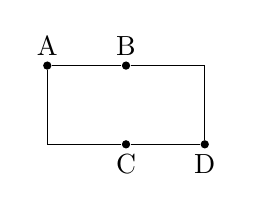
\begin{tikzpicture}
%\draw[step=0.5cm, very thin,black!20] (-3,-3) grid (3,3);
\draw (0,1) node[dot] (A) {} node [above] {A};
\draw (1,1) node[dot] (B) {} node [above] {B};
\draw (1,0) node[dot] (C) {} node [below] {C};
\draw (2,0) node[dot] (D) {} node [below] {D};
\draw (A)--(B)--(2,1)--(D);
\draw (A)--(0,0)--(C)--(D);
\end{tikzpicture}


%\todo[inline]{Рисунок моста}

\begin{enumerate}
\item Сколько машин и по какой дороге едет в равновесии  Нэша?
Сколько им требуется времени, чтобы добраться из $A$ в $D$?
\item  Как изменятся ответы, если между городами $B$ и $C$ построен удобный мост, такой что $f_{BC}=0$?
\end{enumerate}


\begin{sol}
Если моста нет, то есть два пути, $ABD$ и $ACD$. В равновесии Нэша каждым путем едут три машины, поэтому в пути они тратят $49$ минут каждая.

Если мост построен, то заметим, что при любом количестве машин путь $BD$ быстрее пути $CD$, а путь $AC$ быстрее пути $AB$. Значит в равновесии Нэша все едут путем $ACBD$ и каждый тратит на него $62$ минуты.

Данный пример является упрощением, но тем не менее демонстрирует, что строительство новой дороги может увеличить количество пробок.
\end{sol}
\end{problem}


\Closesolutionfile{solution_file}
